%%%% main.tex, 2022/08/10, 2.5
%%%% Copyright (C) 2020 Vinicius Pegorini (vinicius@utfpr.edu.br)
%%
%% This work may be distributed and/or modified under the conditions of the
%% LaTeX Project Public License, either version 1.3 of this license or (at your
%% option) any later version.
%% The latest version of this license is in
%%   http://www.latex-project.org/lppl.txt
%% and version 1.3 or later is part of all distributions of LaTeX version
%% 2005/12/01 or later.
%%
%% This work has the LPPL maintenance status `maintained'.
%%
%% The Current Maintainer of this work is Vinicius Pegorini.
%%
%% This work consists of the files utfprpb.cls, utfprpb.tex, and
%% utfprpb-dados.tex.
%%
%% The Current Maintainer of this work is Vinicius Pegorini.
%% Updated by:
%% - Marco Aurélio Graciotto Silva;
%% - Rogério Aparecido Gonçalves;
%% - Luiz Arthur Feitosa dos Santos.
%%
%% This work consists of the files utfpr.cls, main.tex, and
%% variaveis.tex.
%% A brief description of this work is in readme.md.

%% ####################################################
%%
%% >> Atenção - Leia isso antes de usar esse template<< 
%%
%% Esse template foi desenvolvido por professores,  com a intenção de ajudar os alunos com as entregas na biblioteca. Não há uma equipe especializada e dedicada mantendo tal template, mas sim professores trabalhando além das suas funções básicas, que são: ensino, pesquisa e extensão.
%
%% Também os mantenedores deste template não são especializados em LaTeX, muito menos em normas da ABNT. Todos que contribuíram com o template fizeram isso visando deixá-lo o mais próximo possível das normas da ABNT e das regras, anseios e expectativas da biblioteca da UTFPR. É muito importante entender que os desenvolvedores do template não têm relação direta com a biblioteca ou com a ABNT. Ou seja, não são os desenvolvedores do template que ditam as regras e normas dos textos que devem ser entregues à biblioteca.

%%É válido informar também, que como não há uma equipe dedicada e especializada, o tempo para colaborar com o template é curto. Desta forma, pode ser que não sejam empregadas as melhores técnicas, métodos e ferramentas para o desenvolvimento do template. Também pode acontecer do template não atender completamente todos os anseios e exigências da ABNT e da biblioteca, pois por exemplo, muitas regras de redação possuem questões interpretativas. Assim, o template sempre estará em contínua evolução e seria extremamente interessante que as pessoas (alunos,  professores,  técnicos e entusiastas) colaborarem com a evolução do template. Toda ajuda será bem vinda! Isso pode ser feito enviando e-mail para os desenvolvedores, desta forma, assim que possível esses vão tentar melhorar o template.

%%O template é apenas mais uma ferramenta para o desenvolvimento de trabalhos para a biblioteca. Todavia, podem existir outros templates LaTeX. Assim como há templates em outros formatos, que não o LaTeX. O mais importante é que qualquer pessoa, utilizando a princípio qualquer ferramenta, pode desenvolver textos que atendem os requisitos da biblioteca apenas estudando, interpretando e seguindo as regras da UTFPR e da ABNT, que estão disponíveis na página Web da instituição. O template é só um facilitador.

%%Por fim,  é necessário entender que infelizmente o ambiente LaTeX pode ser complexo e gerar resultados distintos dependendo do: sistema operacional,  pacotes LaTeX utilizados,  configurações alteradas, editor utilizado, a forma que está sendo redigida textos, figuras,  etc. Assim não há como garantir que o resultado final será o esperado.  Dito tudo isso,  >>UTILIZE ESSE TEMPLATE POR SUA CONTA E RISCO<<. Os desenvolvedores e colaboradores deste template não se responsabilizam pelo resultado do uso deste template e se eximem de qualquer responsabilidade.

%###################################################


% Luiz - pdfa: inclusão do pdfa
\PassOptionsToPackage{
	pdfa
}{hyperref}



%% Classe e opções de documento
\documentclass[%% Opções
%% -- Opções da classe memoir --
  12pt,%% Tamanho da fonte: 10pt, 11pt, 12pt, etc.
  a4paper,%% Tamanho do papel: a4paper (A4), letterpaper (carta), etc.
  % fleqn,%% Alinhamento das equações à esquerda (comente para alinhamento centralizado)
  % leqno,%% Numeração das equações no lado esquerdo (comente para lado direito)
  oneside,%% Impressão dos elementos textuais e pós-textuais: oneside (anverso) ou twoside (anverso e verso, se mais de 100 p.)
  openright,%% Impressão da primeira página dos capítulos: openright (anverso), openleft (verso) ou openany (anverso e verso)
%% -- Opções da classe abntex2 --
  sumario = abnt-6027-2012,%% Formatação do sumário: tradicional (estilo tradicional) ou abnt-6027-2012 (norma ABNT 6027-2012)
  chapter = TITLE,%% Títulos de capítulos em maiúsculas (comente para desabilitar)
  % luiz - comentar section para ser minusculo
  %section = TITLE,%% Títulos de seções secundárias em maiúsculas (comente para desabilitar)
  % subsection = TITLE,%% Títulos de seções terciárias em maiúsculas (comente para desabilitar)
  % subsubsection = TITLE,%% Títulos de seções quartenárias em maiúsculas (comente para desabilitar),
%% -- Opções da classe utfprpgtex --
  pretextualoneside,%% Impressão dos elementos pré  -textuais: pretextualoneside (anverso) ou pretextualtwoside (anverso e verso)
  fontetimes,%% Fonte do texto: fontetimes (times), fontearial (arial) ou fontecourier (courier)
  % vinculoscoloridos,%% Cores nos vínculos (citações, arquivos, links, url, etc.) (comente para desabilitar)
  semrecuonosumario,%% Remoção do recuo dos itens no sumário (comente para adição do recuo, se estilo tradicional)
  usemakeindex,%% Compilação de glossários e índices utilizando makeindex (comente para desabilitar)
  % legendascentralizadas,%% Alinhamento das legendas centralizado (comente para alinhamento à esquerda)
  %aprovacaoestiloppg,%% Folha de aprovação do programa de pós-graduação no estilo do PPG (comente para estilo padrão)
  pardeassinaturas,%% Assinaturas na folha de aprovação em até duas colunas (comente para em uma única coluna)
  % linhasdeassinaturas,%% Linhas de assinaturas na folha de aprovação (comente para remover as linhas)
%% -- Opções do pacote babel --
  english,%% Idioma adicional para hifenização
  french,%% Idioma adicional para hifenização
  spanish,%% Idioma adicional para hifenização
  brazil,%% Idioma principal do documento (último da lista)
]{utfpr}%% Classe utfpr

% Luiz: pdfa: necessário para criar pdfa
\usepackage[a-3b,mathxmp]{pdfx}[2018/12/22] % você pode escolher entre a-1b, a-2b, a-3b - o template ainda não suporta o a-Xa de 

%%%% configuracoes.tex, 2022/05/02, 2.4a

%% ####################################################
%%
%% >> Atenção - Leia isso antes de usar esse template<< 
%%
%% Esse template foi desenvolvido por professores,  com a intenção de ajudar os alunos com as entregas na biblioteca. Não há uma equipe especializada e dedicada mantendo tal template, mas sim professores trabalhando além das suas funções básicas, que são: ensino, pesquisa e extensão.
%
%% Também os mantenedores deste template não são especializados em LaTeX, muito menos em normas da ABNT. Todos que contribuíram com o template fizeram isso visando deixá-lo o mais próximo possível das normas da ABNT e das regras, anseios e expectativas da biblioteca da UTFPR. É muito importante entender que os desenvolvedores do template não têm relação direta com a biblioteca ou com a ABNT. Ou seja, não são os desenvolvedores do template que ditam as regras e normas dos textos que devem ser entregues à biblioteca.

%%É válido informar também, que como não há uma equipe dedicada e especializada, o tempo para colaborar com o template é curto. Desta forma, pode ser que não sejam empregadas as melhores técnicas, métodos e ferramentas para o desenvolvimento do template. Também pode acontecer do template não atender completamente todos os anseios e exigências da ABNT e da biblioteca, pois por exemplo, muitas regras de redação possuem questões interpretativas. Assim, o template sempre estará em contínua evolução e seria extremamente interessante que as pessoas (alunos,  professores,  técnicos e entusiastas) colaborarem com a evolução do template. Toda ajuda será bem vinda! Isso pode ser feito enviando e-mail para os desenvolvedores, desta forma, assim que possível esses vão tentar melhorar o template.

%%O template é apenas mais uma ferramenta para o desenvolvimento de trabalhos para a biblioteca. Todavia, podem existir outros templates LaTeX. Assim como há templates em outros formatos, que não o LaTeX. O mais importante é que qualquer pessoa, utilizando a princípio qualquer ferramenta, pode desenvolver textos que atendem os requisitos da biblioteca apenas estudando, interpretando e seguindo as regras da UTFPR e da ABNT, que estão disponíveis na página Web da instituição. O template é só um facilitador.

%%Por fim,  é necessário entender que infelizmente o ambiente LaTeX pode ser complexo e gerar resultados distintos dependendo do: sistema operacional,  pacotes LaTeX utilizados,  configurações alteradas, editor utilizado, a forma que está sendo redigida textos, figuras,  etc. Assim não há como garantir que o resultado final será o esperado.  Dito tudo isso,  >>UTILIZE ESSE TEMPLATE POR SUA CONTA E RISCO<<. Os desenvolvedores e colaboradores deste template não se responsabilizam pelo resultado do uso deste template e se eximem de qualquer responsabilidade.

%###################################################

%% Pacotes carregados nas classes:
%%   memoir: abstract, appendix, array, booktabs, ccaption, chngcntr, chngpage, dcolumn, delarray, enumerate, epigraph, framed,
%%           ifmtarg, ifpdf, index, makeidx, moreverb, needspace, newfile, nextpage, parskip, patchcmd, setspace, shortvrb, showidx,
%%           tabularx, titleref, titling, tocbibind, tocloft, verbatim, verse.
%%   memoir (similares): crop, fancyhdr, geometry, sidecap, subfigure, titlesec.
%%   abntex2: babel, bookmark, calc, enumitem, ifthen, hyperref, textcase.
%%   utfprpgtex: abntex2cite, ae, algorithmic, amsmath, backref, breakurl, caption, cmap, color, eepic, epic, epsfig, etoolbox,
%%               fancyhdr, fix-cm, fontenc, glossaries, graphics, graphicx, helvet, hyphenat, indentfirst, inputenc, lastpage,
%%               morewrites, nomencl, sfmath, sistyle, substr, times, xtab.


%% Pacotes adicionais (\usepackage[options]{package})
\usepackage{bigdelim, booktabs, colortbl, longtable, multirow}%% Ferramentas para tabelas
\usepackage{amssymb, amstext, amsthm, icomma}%% Ferramentas para linguagem matemática
\usepackage{pifont, textcomp, wasysym}%% Símbolos de texto
\usepackage{lipsum}				% para geração de dummy text
\usepackage{subfig}             % para adicionar figuras lado a lado no texto                    
\usepackage{pdfpages}           % para adicionar documentos pdf ao trabalho
\usepackage{xspace}
\usepackage{graphicx}

% luiz: primeira letra maiúscula
% solução 1
%\usepackage{stringstrings}
%\newcommand{\firstcap}[1]{\caselower[e]{#1}\capitalize{\thestring}}

% solução 2 - não usei essa
% \usepackage[utf8]{inputenc}
% \usepackage{datatool-base}
% \usepackage{mfirstuc}

% Formatação do título da seção - primeira letra caixa alta e o resto em caixa baixa.
% \usepackage[explicit]{titlesec}
% \usepackage{lipsum}
% \titleformat{\section}{\normalfont}{\thesection}{1em}{\textbf{\firstcap{#1}}} % funciona mas apenas para o título da seção e não para o sumário (a configuração do sumário está mais para baixo

% luiz: define o underline colorido.
% https://github.com/abntex/abntex2-contrib/blob/master/customizacoes/pucminas/abntex2-pucminas.sty
% acabei não usando o black e o coloruline da solução do link

\usepackage[normalem]{ulem} % para o underline colorido na seção quaternária
\renewcommand*{\cftsubsubsectionfont}{\normalfont\uline} % underline no sumário
\setsubsubsecheadstyle{\ABNTEXsubsubsectionfont\ABNTEXsubsubsectionfontsize\ABNTEXsubsubsectionupperifneeded\uline} %underline no título da subsubsection

% luiz: bibliografia - opções

%% Comandos personalizados (\newcommand{name}[num]{definition})
\newcommand{\cpp}{\texttt{C$++$}}%% C++
\newcommand{\latex}{\LaTeX\xspace}%% LaTeX
\newcommand{\ds}{\displaystyle}%% Tamanho normal das equações
\newcommand{\bsym}[1]{\boldsymbol{#1}}%% Texto no modo matemático em negrito
\newcommand{\mr}[1]{\mathrm{#1}}%% Texto no modo matemático normal (não itálico)
\newcommand{\der}{\mr{d}}%% Operador diferencial
\newcommand{\deri}[2]{\frac{\der #1}{\der #2}}%% Derivada ordinária
\newcommand{\derip}[2]{\frac{\partial #1}{\partial #2}}%% Derivada parcial
\newcommand{\pare}[1]{\left( #1 \right)}%% Parênteses
\newcommand{\colc}[1]{\left[ #1 \right]}%% Colchetes
\newcommand{\chav}[1]{\left\lbrace #1 \right\rbrace}%% Chaves
\newcommand{\sen}{\operatorname{sen}}%% Operador seno
\newcommand{\senh}{\operatorname{senh}}%% Operador seno hiperbólico
\newcommand{\tg}{\operatorname{tg}}%% Operador tangente
\newcommand{\tgh}{\operatorname{tgh}}%% Operador tangente hiperbólico
\newcommand{\seqref}[1]{Equação~\eqref{#1}}%% Referência de uma única equação
\newcommand{\meqref}[1]{Equações~\eqref{#1}}%% Referência de múltiplas equações
\newcommand{\citep}[1]{\cite{#1}}%% Atalho para citação implícita
\newcommand{\citet}[1]{\citeonline{#1}}%% Atalho para citação explícita
\newcommand{\citepa}[1]{(\citeauthor{#1})}%% Atalho para citação implícita (somente autor)
\newcommand{\citeta}[1]{\citeauthoronline{#1}}%% Atalho para citação explícita (somente autor)
\newcommand{\citepy}[1]{(\citeyear{#1})}%% Atalho para citação implícita (somente ano)
\newcommand{\citety}[1]{\citeyear{#1}}%% Atalho para citação explícita (somente ano)

\newcommand{\fonteTexto}[1]{\renewcommand{\familydefault}{#1}}

% Define o caminho das figuras
\graphicspath{{figuras/}}

% Define a fonte ara helvet que é uma fonte similar à Arial, se for usar a Arial tem que mudar o compilador para XeLaTex, mas ai tem que arrumar os erros: https://latex.org/forum/viewtopic.php?t=25998
%\usepackage{helvet}
%\renewcommand{\familydefault}{\sfdefault}
%\usepackage{times} % para fonte time new roman
%\usepackage{pslatex} % ou essa aqui...

%\usepackage{titlesec}

%% Configuração de glossário
% \usepackage[portuguese]{nomencl}
% \usepackage[nogroupskip,nonumberlist,nopostdot,nohypertypes={acronym}]{glossaries}
% \makenoidxglossaries
\usepackage{glossaries}
\makeglossaries

% para siglas em português
\newcommand{\siglaPt}[2]
{
    \newglossaryentry{#1}{
        name=#1,
        description={#2},
        first={#2 (#1)},
        long={#2}
    }
}

% para siglas de língua estrangeira, nessas a descrição longa fica em itálico.
\newcommand{\siglaIt}[2]
{
    \newglossaryentry{#1}{
        name=#1,
        description={\textit{#2}},
        first={\textit{#2} ({#1})},
        long={\textit{#2}}
    }
}

%% luiz - para fazer os avisos
\usepackage{tcolorbox}

% use para criar caixas de avisos, pode ser utilizado para fazer anotações de tarefas indicadas pelo orientador/banca.
% \caixa{Atenção}{texto...}
\newcommand{\caixa}[2]{
    \begin{tcolorbox}[colback=red!5!white,colframe=red!45!white, title = #1, fonttitle=\bfseries]
        #2
    \end{tcolorbox}
}

% Luiz - Linhas órfãs e viúvas
\widowpenalty=10000
\clubpenalty=10000

% Luiz - Caption do tamanho da Tabela
%\usepackage[width=1\textwidth]{caption}

% Luiz - configurar a margem dos itens
\setlength{\leftmargini}{1.5cm}
\setlength{\leftmarginii}{1.5cm}


%% Arquivo de dados do modelo de documento LaTeX para produção de trabalhos acadêmicos da UTFPR
%%%% variaveis.tex, 2022/05/02, 2.4a
%%%% Copyright (C) 2020 Vinicius Pegorini (vinicius@utfpr.edu.br)
%%
%% This work may be distributed and/or modified under the conditions of the
%% LaTeX Project Public License, either version 1.3 of this license or (at your
%% option) any later version.
%% The latest version of this license is in
%%   http://www.latex-project.org/lppl.txt
%% and version 1.3 or later is part of all distributions of LaTeX version
%% 2005/12/01 or later.
%%
%% This work has the LPPL maintenance status `maintained'.
%%
%% The Current Maintainer of this work is Vinicius Pegorini.
%% Updated by:
%% - Marco Aurélio Graciotto Silva;
%% - Rogério Aparecido Gonçalves;
%% - Luiz Arthur Feitosa dos Santos.
%%
%% This work consists of the files utfpr.cls, main.tex, and
%% variaveis.tex.
%%
%% A brief description of this work is in readme.txt.

%% ####################################################
%%
%% >> Atenção - Leia isso antes de usar esse template<< 
%%
%% Esse template foi desenvolvido por professores,  com a intenção de ajudar os alunos com as entregas na biblioteca. Não há uma equipe especializada e dedicada mantendo tal template, mas sim professores trabalhando além das suas funções básicas, que são: ensino, pesquisa e extensão.
%
%% Também os mantenedores deste template não são especializados em LaTeX, muito menos em normas da ABNT. Todos que contribuíram com o template fizeram isso visando deixá-lo o mais próximo possível das normas da ABNT e das regras, anseios e expectativas da biblioteca da UTFPR. É muito importante entender que os desenvolvedores do template não têm relação direta com a biblioteca ou com a ABNT. Ou seja, não são os desenvolvedores do template que ditam as regras e normas dos textos que devem ser entregues à biblioteca.

%%É válido informar também, que como não há uma equipe dedicada e especializada, o tempo para colaborar com o template é curto. Desta forma, pode ser que não sejam empregadas as melhores técnicas, métodos e ferramentas para o desenvolvimento do template. Também pode acontecer do template não atender completamente todos os anseios e exigências da ABNT e da biblioteca, pois por exemplo, muitas regras de redação possuem questões interpretativas. Assim, o template sempre estará em contínua evolução e seria extremamente interessante que as pessoas (alunos,  professores,  técnicos e entusiastas) colaborarem com a evolução do template. Toda ajuda será bem vinda! Isso pode ser feito enviando e-mail para os desenvolvedores, desta forma, assim que possível esses vão tentar melhorar o template.

%%O template é apenas mais uma ferramenta para o desenvolvimento de trabalhos para a biblioteca. Todavia, podem existir outros templates LaTeX. Assim como há templates em outros formatos, que não o LaTeX. O mais importante é que qualquer pessoa, utilizando a princípio qualquer ferramenta, pode desenvolver textos que atendem os requisitos da biblioteca apenas estudando, interpretando e seguindo as regras da UTFPR e da ABNT, que estão disponíveis na página Web da instituição. O template é só um facilitador.

%%Por fim,  é necessário entender que infelizmente o ambiente LaTeX pode ser complexo e gerar resultados distintos dependendo do: sistema operacional,  pacotes LaTeX utilizados,  configurações alteradas, editor utilizado, a forma que está sendo redigida textos, figuras,  etc. Assim não há como garantir que o resultado final será o esperado.  Dito tudo isso,  >>UTILIZE ESSE TEMPLATE POR SUA CONTA E RISCO<<. Os desenvolvedores e colaboradores deste template não se responsabilizam pelo resultado do uso deste template e se eximem de qualquer responsabilidade.

%###################################################

%% Documento
%% Luiz: Define a fonte do texto da monografia
\fonteTexto{\sfdefault} % utilize \rmdefault para Times New Roman ou \sfdefault para Arial
\TipoDeDocumento{Trabalho de Conclusão de Curso de Graduação}%% Tipo de documento: "Tese", "Dissertação" ou "Trabalho de Conclusão de Curso de Graduação", "Estágio Supervisionado"
\NivelDeFormacao{Bacharelado}%% Nível de formação: "Doutorado", "Mestrado", "Bacharelado" ou "Tecnólogo" - ATENÇÃO, isso será utilizado para alterar a formatação do trabalho, pois pode haver formatações distintas dependendo o nível/tipo de trabalho.


%% luiz
% Template LaTex criado pelo Departamento Acadêmico de Computação (DACOM)
% da Universidade Tecnológica Federal do Paraná - Campus Campo Mourão (UTFPR-CM)
% Criado e alterado pelos professores:
% - Marco Aurélio Graciotto Silva
% - Rogério Aparecido Gonçalvez
% - Luiz Arthur Feitosa dos Santos
% Esse template utiliza a licença CC BY:
% Esta licença permite que outros distribuam, remixem, adaptem e criem a partir deste trabalho, mesmo para fins comerciais, desde que atribuam o devido crédito pela criação original.
% https://creativecommons.org/licenses/by/4.0/deed.pt_BR

% Dados do curso. Caso seja BCC:
\program{Curso de Bacharelado em Ciência da Computação}
\programen{Undergradute Program in Computer Science}
\degree{Bacharel}
\degreearea{Ciência da Computação}
% Caso seja TSI:
% \program{Curso Superior de Tecnologia em Sistemas para Internet}
% \programen{Undergradute Program in Tecnology for Internet Systems}
% \degree{Tecnólogo}
% \degreearea{Tecnologia em Sistemas para Internet}


% Dados da disciplina. Escolha uma das opções e a descomente:
% TCC1:
\goal{Proposta de Trabalho de Conclusão de Curso de Graduação}
\course{Trabalho de Conclusão de Curso 1}
% TCC2:
%\goal{Trabalho de Conclusão de Curso de Graduação}
%\course{Trabalho de Conclusão de Curso 2}


% Dados do TCC (precisa alterar)
\author{JOÃO VICTOR BRIGANTI DE OLIVEIRA}  % Seu nome
\authorbib{Briganti, João} % Seu nome para referência bibliográfica (Sobrenome, Nome)
\title{Extensão do OpenMP para Suporte de Técnicas de Aproximação}

\titleFA{Extensão do OpenMP para Suporte de Técnicas de Aproximação}

\titleen{OpenMP Extension for Approximate Computing Techniques} % Título traduzido para inglês
\advisor{Prof. Dr. João Fabrício Filho} % Nome do orientador. Lembre-se de prefixar com "Prof. Dr.", "Profª. Drª.", "Prof. Me." ou "Profª. Me."}
% Se não houver corientador, comente a linha a baixo
\coadvisor{Prof. Dr. Rogério Aparecido Gonçalves} % Nome do coorientador, caso exista. Caso não exista, comente a linha.
\depositshortdate{2025} % Ano em que depositou este documento
\approvaldate{dia / mês por extenso / ano}

% Dados do curso que não precisam de alteração
\university{Universidade Tecnológica Federal do Paraná}
\universityen{Federal University of Technology -- Paraná}
\universitycampus{Campus Campo Mourão}
\universityunit{Departamento Acadêmico de Computação}
\address{CAMPO MOURÃO}
\addressen{Campus Cornélio Procópio, PR, Brazil}
\documenttype{Monografia}
\documenttypeen{Monograph}
\degreetype{Graduação}

\evalboardmember{Nome completo e por extenso do Membro 1 (de acordo com o Currículo Lattes)
}{Titulação (Especialização, Mestrado, Doutorado)}{Nome completo e por extenso da instituição a qual possui vínculo}
\evalboardmember{Nome completo e por extenso do Membro 2 (de acordo com o Currículo Lattes)
}{Titulação (Especialização, Mestrado, Doutorado)}{Nome completo e por extenso da instituição a qual possui vínculo}
\evalboardmember{Nome completo e por extenso do Membro 3 (de acordo com o Currículo Lattes)
}{Título (Titulação (Especialização, Mestrado, Doutorado)}{Nome completo e por extenso da instituição a qual possui vínculo}
%\evalboardmember{Nome completo e por extenso do Membro 4}{Título (especialização, mestrado, doutorado}{Nome completo e por extenso da instituição a qual possui vínculo}

%% Palavras-chave e keywords
%% ATENÇÃO - você deve indicar a quantidade de palavras chaves para o template LaTeX utilizar o pontuação correta!
\NumeroDePalavrasChave{3}%% Número de palavras-chave (máximo 5)
%% Atenção - por enquanto o template não está suportando acentos normais na palavra chave, por isso caso a palavra tenha acento, você deve utilizar o estilo antigo do LaTeX, sendo os acentos: á - \'a  é - \'e   â - \^a  ê - \^e  à - \`a  ä - \"a  ç - \c{c}
\PalavraChaveA{paralelismo}%% Palavra-chave A
\PalavraChaveB{LLVM}%% Palavra-chave B
\PalavraChaveC{alto desempenho}%% Palavra-chave C
%\PalavraChaveD{palavra 4}%% Palavra-chave D
%\PalavraChaveE{Palavra-chave 5}%% Palavra-chave E
%% Exemplo de como utilizar acentos na Palavra-chave:
% \PalavraChaveA{ol\'a}%% Olá
%\PalavraChaveB{voc\^e}%% você
%\PalavraChaveC{\`a}%% à
%\PalavraChaveD{a\c{c}\~ao}%% ação
%\PalavraChaveE{arg\"uir}%% argüir


%% ATENÇÃO - você deve indicar a quantidade de keywords para o template LaTeX utilizar o pontuação correta!
\NumeroDeKeywords{3}%% Número de keywords (máximo 5)
\KeywordA{parallelism}%% Keyword A
\KeywordB{LLVM}%% Keyword B
\KeywordC{high performance}%% Keyword C
%\KeywordD{word 4}%% Keyword D
%\KeywordE{Keyword 5}%% Keyword E


% É obrigatório o uso de uma licença Creative Commons (CC) nos trabalhos de TCC pelos cursos ligados a DACOM da UTFPR-CM.
% Veja: http://portal.utfpr.edu.br/biblioteca/trabalhos-academicos/docentes/procedimento-de-entrega-graduacao

% Sendo assim, escolha com o seu orientador uma das licenças CC a seguir: 

% CC BY: Esta licença permite que outros distribuam, remixem, adaptem e criem a partir deste trabalho, mesmo para fins comerciais, desde que atribuam o devido crédito pela criação original. Essa é a menos restritiva.
\licenca{ccby}

% CC BY CA: Esta licença permite que outros remixem, adaptem e criem a partir deste trabalho, mesmo para fins comerciais, desde que atribuam o devido crédito e que licenciem as novas criações sob termos idênticos.
%\licenca{ccbysa}

% CC BY ND: Esta licença permite a redistribuição, comercial e não comercial, desde que o trabalho seja distribuído inalterado e no seu todo, com crédito ao autor.
%\licenca{ccbynd}

% CC BY NC: Esta licença permite que outros remixem, adaptem e criem a partir deste trabalho para fins não comerciais, e embora os novos trabalhos tenham de atribuir o devido crédito e não possam ser usados para fins comerciais, os trabalhos derivados não têm que serem licenciados sob os mesmos termos.
%\licenca{ccbync}

% CC BY NC SA: Esta licença permite que outros remixem, adaptem e criem a partir deste trabalho para fins não comerciais, desde que atribuam ao autor o devido crédito e que licenciem as novas criações sob termos idênticos.
%\licenca{ccbyncsa}

% CC BY NC ND: Esta licença só permite que outros façam download do trabalho e o compartilhe desde que atribuam crédito ao autor, mas sem que possam alterá-los de nenhuma forma ou utilizá-los para fins comerciais. Essa é a mais restritiva.
%\licenca{ccbyncnd}

% Deixar sem licença - isso é aplicado apenas aos trabalhos que não são obrigados a ter licença. Na duvida verifique isso com o seu orientador e professor responsável pelo TCC. Para deixar o texto sem licença deixe o comando licença em brando ou deixe comentado.
%\licenca{}
% by DACOM/UTFPR-CM%% Realize as modificações pertinentes no arquivo "utfprpb-dados.tex"

%% Ferramenta para criação de índices
\makeindex%% Não comente esta linha

%% Ferramenta para criação de glossários
\makeglossaries%% Não comente esta linha
%%%% LISTA DE ABREVIATURAS E SIGLAS 
%%
%% Relação, em ordem alfabética, das abreviaturas (representação de uma palavra por meio de alguma(s) de sua(s) sílaba(s) ou
%% letra(s)), siglas (conjunto de letras iniciais dos vocábulos e/ou números que representa um determinado nome) e acrônimos
%% (conjunto de letras iniciais dos vocábulos e/ou números que representa um determinado nome, formando uma palavra pronunciável).
%%
%% Este arquivo para definição de abreviaturas, siglas e acrônimos é utilizado com a opção "glossaries" (pacote)

%% Abreviaturas: \abreviatura{rótulo}{representação}{definição}

\abreviatura{art.}{art.}{Artigo}
\abreviatura{cap.}{cap.}{Capítulo}
\abreviatura{sec.}{sec.}{Seção}

%% Siglas: \sigla{rótulo}{representação}{definição}

\sigla{ca}{CA}{Computação Aproximada}
\sigla{simd}{SIMD}{\textit{Single Instruction Multiple Data}}
\sigla{gpu}{GPU}{\textit{Graphics Processing Unit}}
\sigla{api}{API}{\textit{Application Programming Interface}}
\sigla{hpc}{HPC}{\textit{High-Performance Computing}}

%% LEIA:

%% Para usar o \gls, você deve colocar a sigla aqui em \sigla

%% ADICIONAR SIGLAS: Quando você inclui alguma sigla, pode ser necessário compilar umas duas vezes para essa aparecer na lista de siglas.

%% ATENÇÃO REMOVER SIGLAS: se você remover a sigla do seu texto (não for usar mais), você deve comentar essa aqui e remover os \gls{} dessa sigla (se não vai ficar aparecendo a sigla na lista). Em caso de ERRO, quando o LaTeX informa que você ainda tem a sigla no texto, mesmo que não tenha. Você deve limpar o cache - no OverLeaf, clique no erro, vá:
%  ->view error
%%   ->(role para baixo, até o final)
%%     ->e clique em Clear cached files


%% Acrônimos: \acronimo{rótulo}{representação}{definição}
%\acronimo{gimp}{Gimp}{Programa de Manipulação de Imagem GNU, do inglês \textit{GNU Image Manipulation Program}}
%% Entradas da lista de abreviaturas e siglas - Comente para remover este item
%%%% GLOSSÁRIO
%%
%% Relação de palavras ou expressões técnicas de uso restrito ou de sentido obscuro, utilizadas no texto, acompanhadas das
%% respectivas definições.

%% Entradas do glossário: \newglossaryentry{rótulo}{informações da entrada}

\newglossaryentry{pai}{%% Informações da entrada
  name        = {pai},
  plural      = {pais},
  description = {um exemplo de entrada pai que possui subentradas (entradas filhas)}
}

\newglossaryentry{componente}{%% Informações da entrada
  name        = {componente},
  plural      = {componentes},
  parent      = {pai},
  description = {um exemplo de uma entrada componente, subentrada da entrada chamada \gls{pai}}
}

\newglossaryentry{filho}{%% Informações da entrada
  name        = {filho},
  plural      = {filhos},
  parent      = {pai},
  description = {um exemplo de uma entrada filha (subentrada) da entrada chamada \gls{pai}. Trata-se de uma entrada irmã da entrada chamada \gls{componente}}
}

\newglossaryentry{equilibrio}{%% Informações da entrada
  name        = {equilíbrio da configuração},
  see         = [veja também]{componente},
  description = {uma consistência entre os \glspl{componente}}
}

\newglossaryentry{tex}{%% Informações da entrada
  name        = {\TeX},
  sort        = {TeX},
  description = {é um sistema de tipografia criado por Donald E. Knuth}
}

\newglossaryentry{latex}{%% Informações da entrada
  name        = {\latex},
  sort        = {LaTeX},
  description = {um conjunto de macros para o processador de textos \gls{tex}, utilizado amplamente para a produção de textos matemáticos e científicos devido à sua alta qualidade tipográfica}
}

\newglossaryentry{bibtex}{%% Informações da entrada
  name        = {Bib\TeX},
  sort        = {BibTeX},
  parent      = {latex},
  description = {um software de gerenciamento de referências para a formatação de listas de referências. A ferramenta Bib\TeX\ é normalmente usada em conjunto com o sistema de preparação de documentos do \gls{latex}}
}

\newglossaryentry{abntex2}{%% Informações da entrada
  name        = {\abnTeX},
  sort        = {abnTeX2},
  see         = {latex},
  description = {uma suíte para \gls{latex} que atende os requisitos das normas da Associação Brasileira de Normas Técnicas (ABNT) para elaboração de documentos técnicos e científicos brasileiros, como artigos científicos, relatórios técnicos, trabalhos acadêmicos como teses, dissertações, projetos de pesquisa e outros documentos do gênero}
}

\newglossaryentry{utfprpbtex}{%% Informações da entrada
  name        = {\utfprpbtex},
  sort        = {UTFPRPBTeX},
  see         = {latex},
  parent      = {abntex2},
  description = {uma suíte para \gls{latex}, baseada na suíte \gls{abntex2}, que atende os requisitos das normas definidas pela Universidade Tecnológica Federal do Paraná (UTFPR), Câmpus Pato Branco, para elaboração de trabalhos acadêmicos}
}
%% Entradas do glossário - Comente para remover este item

%% Ferramenta para criação de nomenclaturas
\makenomenclature%% Não comente esta linha

%% Início do documento
\begin{document}%% Não comente esta linha

%% Formatação de páginas de elementos pré-textuais
\pretextual%% Não comente esta linha

%% Capa
%\incluircapa%% Comente para remover este item
\coverpageone

%% Folha de rosto (* coloca a ficha bibliográfica no verso)
%\incluirfolhaderosto*%% Comente para remover este item
\coverpagetwo

% luiz - iniciar contagem depois da folha de rosto
\clearpage
\setcounter{page}{2}

%% Ficha catalográfica (teses e dissertações)
%\incluirfichacatalografica%% Comente para remover este item

%% Errata
%%%%% ERRATA
%%
%% Lista dos erros ocorridos no texto, seguidos das devidas correções.

\begin{errata}%% Ambiente errata
\begin{table*}[htb]%% Ambiente table
\begin{tabularx}{\textwidth}{|l|l|X|X|}%% Ambiente tabularx
\hline
\textbf{Página(s)}         & \textbf{Linha(s)} & \textbf{Onde se lê} & \textbf{Leia-se}         \\ \hline
\pageref*{errata:capitulo} & 4, 9-11, 14-16    & capítulo(s)         & seção(ões) primária(s)   \\ \hline
\pageref*{errata:secao}    & 12-16             & seção(ões)          & seção(ões) secundária(s) \\ \hline
\pageref*{errata:subsecao} & 16                & subseção(ões)       & seção(ões) terciária(s)  \\ \hline
\end{tabularx}
\end{table*}
\end{errata}
%% Comente para remover este item

%% Folha de aprovação
%\incluirfolhaaprovacao
\approvalpage
%\incluirfolhadeaprovacao%% Para adicionar no formato de texto
%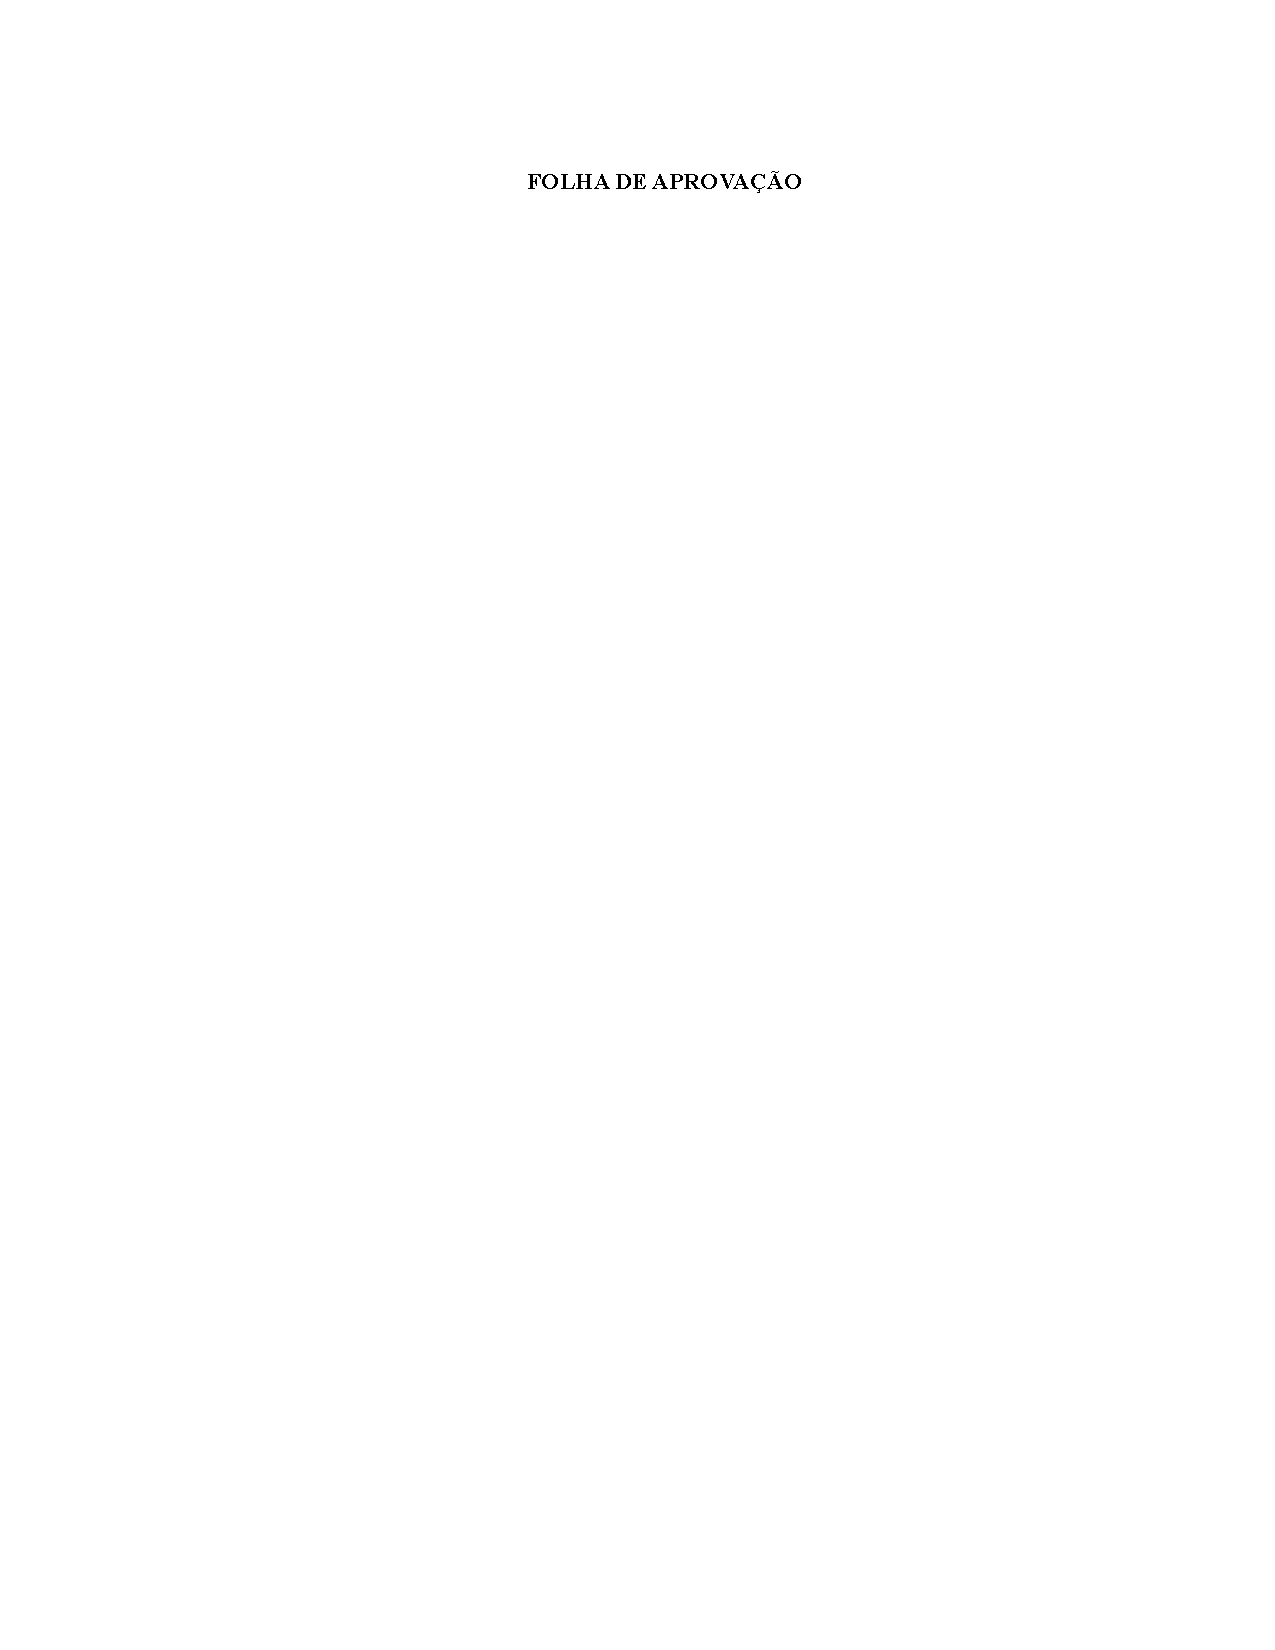
\includepdf[scale=1.0,pages=1]{./PreTexto/folha-aprovacao.pdf} % para adicionar o pdf enviado pelo professor apenas substitua o documento folha-aprovacao.pdf dentro da pasta PreTexto

%% Dedicatória
%%%% DEDICATÓRIA
%%
%% Texto em que o autor presta homenagem ou dedica seu trabalho.

\begin{dedicatoria}%% Ambiente dedicatoria

%Espaço destinado à dedicatória (elemento opcional). Folha que contém o oferecimento do trabalho à determinada pessoa ou pessoas. Exemplo:



Dedico este trabalho à minha família, pelos momentos de ausência.

\end{dedicatoria}
%% Comente para remover este item

%% Agradecimentos
\begin{agradecimentos}%% Ambiente agradecimentos
    Primeiramente, agradeço a minha família, em especial ao meu pai e minha mãe, que foram meu grande apoio ao longo de toda essa jornada, sem os seus ensinamentos e apoio nada disso seria possível.

    Agradeço aos meus orientadores Prof. Dr. João Fabrício Filho e ao Prof. Dr. Rogério Aparecido Gonçalves, pelas suas orientações e contribuições valiosas, não só neste trabalho como também ao longo de toda minha Iniciação Científica.

    Também agradeço a minha namorada pela sua companhia e estar ao meu lado nos momentos dificéis.

    Enfim, agradeço a todos que direta ou indiretamente me ajudaram e estiveram no meu lado durante minha caminhada.
\end{agradecimentos}
%% Comente para remover este item

%% Epígrafe
%%%% EPÍGRAFE
%%
%% Texto em que o autor apresenta uma citação, seguida de indicação de autoria, relacionada com a matéria tratada no corpo do
%% trabalho.

\begin{epigrafe}%% Ambiente epigrafe
%
%Espaço destinado à epígrafe (elemento opcional). Nesta folha, o(a) autor(a) usa uma citação, seguida de indicação de autoria e ano, relacionada, preferencialmente, com o assunto tratado no corpo do trabalho. A citação deverá constar na lista de referências. Exemplo: 
%
``A biblioteca é um jardim onde as ideias florescem e os frutos são colhidos pela eternidade.'' \cite{Candido2002}.
\end{epigrafe}
%% Comente para remover este item

%% Resumo
\begin{resumoutfpr}
    Com o fim da Lei de Moore e da escala de Dennard, diferentes técnicas computacionais surgiram para suprir a demanda por maior desempenho computacional e eficiência energética. A Computação Aproximada é um paradigma que visa aumentar o desempenho e a eficiência energética de aplicações em troca de pequenas perdas de precisão. A Computação Paralela também surge como um paradigma de computação que busca obter maior desempenho por meio de um melhor aproveitamento dos processadores \textit{multicore}. O \texttt{OpenMP} surge como uma ferramenta desse paradigma, facilitando o desenvolvimento de aplicações paralelas por meio de anotações de código. A proposta deste trabalho é implementar diferentes técnicas de aproximação no \texttt{OpenMP} por meio de modificações em sua infraestrutura no LLVM. As técnicas propostas são: perfuração de laços, memoização aproximada, descarte de tarefas e relaxamento de ponto flutuante. As técnicas propostas foram avaliadas utilizando um \textit{benchmark suite} composto pelas aplicações \textit{K-Means}, \textit{2MM}, \textit{Correlação}, \textit{Deriche}, \textit{Jacobi 2D}, \textit{Mandelbrot} e \textit{PI de Monte Carlo}.
\end{resumoutfpr}

%De acordo com a NBR 6028:2021, a apresentação gráfica deve seguir o padrão do documento no qual o resumo está inserido. Para definição das palavras-chave (e suas correspondentes em inglês no abstract) consultar em Termo tópico do Catálogo de Autoridades da Biblioteca Nacional, disponível em: http://acervo.bn.gov.br/sophia_web/autoridade%% Comente para remover este item

%% Abstract
%%%% ABSTRACT
%%
%% Versão do resumo para idioma de divulgação internacional.

\begin{abstractutfpr}%% Ambiente abstractutfpr
Seguir o mesmo padrão do resumo, com a tradução do texto do resumo e referência, se houver, para a língua estrangeira (língua inglesa).
\end{abstractutfpr}
%% Comente para remover este item

%% Lista de algoritmos
%\incluirlistadealgoritmos%% Comente para remover este item


%% Lista de Ilustrações
%% Figuras, Gráficos, Quadros e Fotografias são incluídos juntos em uma mesma lista
%% Na UTFPR sugere-se adotar listas próprias, conforme a natureza da ilustração, a partir da existência de 3 elementos da mesma natureza.Neste caso, cada lista deverá iniciar em folha distinta. Não criar listas com apenas um item.


\incluirlistadeilustracoes


%% Lista de figuras
%\incluirlistadefiguras%% Comente para remover este item

%\incluirlistageraldeilustracoes
%\listofgeneralilust



%% Lista de Fotografias
%\incluirlistadefotografias %% Comente para remover este item


%% Lista de Gráficos
%\incluirlistadegraficos %% Comente para remover este item

%% Lista de tabelas
\incluirlistadetabelas%% Comente para remover este item

%% Lista de quadros
%\incluirlistadequadros

%% Listagem de códigos fonte
%\incluirlistadecodigosfonte

%% Lista de abreviaturas, siglas e acrônimos
\incluirlistadeacronimos{glossaries}%% Opções: "glossaries" (pacote) ou "file" (arquivo) ou "none" (desabilita)

%% Lista de símbolos
\incluirlistadesimbolos{file}%% Opções: "nomencl" (pacote) ou "file" (arquivo) ou "none" (desabilita)

%% Sumário
\incluirsumario%% Comente para remover este item

%% Formatação de páginas de elementos textuais
\textual%% Não comente esta linha

%% Parte
% \part{Introdução}%% Comente para remover este item

%% Capítulo introdução - obrigatório
\chapter{Introdução}\label{cap:introducao}

Por décadas, a Lei de Moore e a escala de Dennard impulsionaram melhorias exponenciais no desempenho computacional e na eficiência energética. A Lei de Moore possibilitou maiores densidades de transistores, enquanto a escala de Dennard garantiu que o consumo de energia permanecesse controlado. À medida que a tecnologia se aproximou de limites fundamentais, ambas as tendências entraram em colapso, tornando os ganhos de desempenho cada vez mais difíceis, hoje limitados a apenas alguns poucos por cento ao ano~\cite{hennessy2019}. Mesmo com essas limitações, a crescente demanda por maior desempenho computacional e eficiência energética tem impulsionado inovações em uma ampla variedade de plataformas, desde sistemas embarcados até \textit{datacenters}. Essa demanda é impulsionada pela crescente complexidade das cargas de trabalho modernas, como análise de dados em tempo real, aprendizado de máquina e processamento de sinais, que frequentemente exigem vastos recursos computacionais~\cite{mittal2016, dalloo2024}.

Para atender a essas demandas sob restrições de desempenho e energia, pesquisadores têm explorado paradigmas alternativos de computação. A \gls{ca} é um paradigma que busca equilibrar precisão computacional e eficiência de recursos. Ela parte do princípio de que muitas aplicações não necessitam de resultados exatos, mas sim de resultados suficientemente precisos dentro de limites aceitáveis, definidos pela percepção do usuário ou por métricas de qualidade específicas~\cite{dalloo2024}. Ao explorar a diferença entre a precisão realmente exigida e a tradicionalmente garantida pelos sistemas, a \gls{ca} viabiliza ganhos expressivos em desempenho, consumo de energia e utilização de \textit{hardware}~\cite{xu2016,leon2025a,leon2025b}.

A \gls{cp} é outro paradigma amplamente adotado nos últimos anos, especialmente com a popularização de processadores \textit{multicore} em computadores pessoais e dispositivos móveis. Essa tendência intensificou a necessidade de desenvolver softwares paralelos, estimulando o surgimento de ferramentas que simplificam a criação dessas aplicações~\cite{goncalves2016}. O \texttt{OpenMP} é uma dessas ferramentas: ele permite que desenvolvedores anotem o código para execução paralela, delegando ao compilador a maior parte da complexidade de gerenciamento~\cite{alrawais2021}. Esse paradigma tornou-se essencial em \gls{hpc}, especialmente em simulações científicas, que tipicamente demandam elevado poder de processamento~\cite{adhikari2012}.

Embora as técnicas de \gls{ca} ofereçam benefícios expressivos, sua aplicação eficaz requer a identificação cuidadosa de regiões de código onde a aproximação seja segura e vantajosa. Esse processo normalmente exige análise detalhada do comportamento da aplicação e de seus requisitos de qualidade~\cite{sampson2015,reis2021}. Este trabalho parte da hipótese de que é possível melhorar o desempenho de aplicações combinando técnicas de aproximação e paralelização, preservando a facilidade de uso provida por ferramentas como o \texttt{OpenMP}. Dessa forma, busca-se explorar simultaneamente os ganhos oferecidos pela execução paralela e pela computação aproximada.

\section{Objetivos}\label{cap:objetivos}

O objetivo geral deste trabalho é melhorar o desempenho de aplicações de \gls{hpc} por meio da aplicação combinada de técnicas de aproximação e paralelização.

Para atingir esse objetivo, foram definidos os seguintes objetivos específicos:
\begin{itemize}
    \item Desenvolver um \textit{benchmark} voltado à avaliação de técnicas de \gls{ca};
    \item Implementar uma extensão do \texttt{OpenMP} com suporte a técnicas de aproximação baseadas em anotações;
    \item Adicionar suporte em tempo de execução para múltiplos algoritmos de aproximação dentro do \texttt{runtime} do \texttt{OpenMP};
    \item Integrar um passo de perfuração de laços ao pipeline de otimização do LLVM;
    \item Realizar a avaliação experimental das técnicas propostas em um ambiente de \gls{ca}.
\end{itemize}

\section{Contribuições}\label{cap:contribuicoes}

As principais contribuições deste trabalho são: o desenvolvimento de um \textit{benchmark suite} voltado à avaliação de \gls{ca}, a implementação de uma extensão do \texttt{OpenMP} com suporte a técnicas de aproximação e a integração dessas funcionalidades à infraestrutura do LLVM. As aplicações que compõem o \textit{benchmark} foram selecionadas com base em conjuntos amplamente utilizados, como o PolyBench~\cite{polybench} e o Debian Benchmarks Game~\cite{debianBenchmarksGame}, e adaptadas para suportar anotações com \texttt{OpenMP}. Também foi implementada uma infraestrutura para avaliação da aceitabilidade dos resultados produzidos. A extensão proposta exigiu modificações na infraestrutura do LLVM, bem como adaptações em algoritmos e escalonadores do \texttt{OpenMP}, a fim de possibilitar o suporte a tarefas aproximadas.

\section{Organização do Trabalho}\label{cap:org_trabalho}

O restante deste trabalho está organizado da seguinte forma: no \autoref{cap:fundamentacaoTeorica} são apresentados os conceitos fundamentais de \gls{ca} e \gls{cp} relacionados a este estudo, incluindo as técnicas de aproximação abordadas — perfuração de laço, memoização aproximada, descarte de tarefas e relaxamento de ponto flutuante, além de uma introdução ao \texttt{OpenMP} e uma revisão de trabalhos correlatos. No \autoref{cap:proposta} é apresentada a proposta dos construtores implementados no \texttt{OpenMP} utilizando a infraestrutura do LLVM. No \autoref{cap:metodologia} são detalhadas a metodologia e as ferramentas empregadas para a realização dos experimentos. Por fim, o \autoref{cap:cronograma} apresenta o cronograma de execução deste trabalho.



%% Capítulo
\chapter{Fundamentaç\~ao Te\'orica}\label{cap:fundamentacaoTeorica}

Este capítulo apresenta os conceitos relacionados a \gls{ca} e Computação Paralela. Primeiramente aborda-se a definição de \gls{ca}, seu uso em aplicações, os desafios enfrentados por essa estratégia e o detalhamento dos algoritmos de perforação de laço, memoização, aproximação de ponto flutuante e o descarte de tarefas. Por fim apresenta também conceitos de Computação Paralela com um foco no uso da ferramenta OpenMP.

\section{Computação aproximada}\label{sec:compAprox}

A \gls{ca} consiste em um conjunto de técnicas aplicadas a cenários em que os resultados exatos não são estritamente necessários ou em que as aplicações apresentam resiliência suficiente para lidar com pequenas imprecisões em suas computações. Nessas situações, o uso de tais técnicas pode proporcionar ganhos significativos de desempenho e eficiência energética, mantendo a margem de erro em níveis reduzidos. Um exemplo é o uso de redes neurais para aproximar a divergência de \textit{branch} em instruções \gls{simd}, capaz de alcançar aceleração de até 14,8$\times$ com acurácia de 96\%~\cite{grigorian2015}. Por esse motivo, a \gls{ca} se mostra especialmente atraente em domínios como análise de dados, reconhecimento de padrões, processamento de imagens e sinais~\cite{mittal2016, chippa2013}.

As diferentes estratégias de aproximação podem ser classificadas conforme a camada em que são aplicadas na pilha computacional. No nível de \textit{hardware}, destacam-se técnicas que envolvem desde unidades funcionais aproximadas, como somadores, multiplicadores e divisores, até abordagens como \textit{overclocking}~\cite{leon2025a,leon2025b} e o uso de memórias aproximadas~\cite{fabricio2020}. No nível de \textit{software}, encontram-se estratégias mais generalistas, incluindo linguagens de programação aproximada~\cite{sampson2015}, \textit{runtimes} com suporte à aproximação~\cite{li2018,reis2024} e otimizações realizadas em nível de compilador~\cite{oliveira2024a,oliveira2024b}.

Apesar de seus benefícios, esse paradigma enfrenta desafios significativos. Em primeiro lugar, nem todas as aplicações são resilientes a erros em sua execução, o que limita o uso de técnicas mais generalistas e torna necessário definir métricas que permitam ajustar o grau de precisão desejado, seja pelo usuário ou pela própria aplicação~\cite{mittal2016}. Além disso, medir corretamente o nível de erro introduzido não é trivial, pois nem sempre está claro qual métrica deve ser aplicada à saída da aplicação~\cite{felzmann2021}. Outro ponto crítico é a propagação dos erros, que pode comprometer toda a execução: em alguns casos, a aplicação pode falhar abruptamente; em outros, concluir sua execução de forma aparentemente correta, mas com resultados significativamente distantes do esperado~\cite{fabricio2020}.

Diante disso é possível observar que a \gls{ca} não se restringe a um único método, mas a um conjunto de diversas estratégias que exploram diferentes aspectos da execução de um programa. Na subseção seguinte, são detalhados quatro dessas estratégias: perforação de laço, memoização, aproximação de ponto flutuante e o descarte de tarefas

\subsection{Perforação de laço}\label{subsec:perfLaco}

A perforação de laço é uma das técnicas mais simples de computação aproximada, cuja ideia central consiste em omitir determinadas iterações de um laço, reduzindo assim o tempo de execução de uma região de código~\cite{sidiroglou2011}.

Existem diferentes forma de implementar esse técnica, existem técnicas estáticas que são aplicadas em tempo de compilação e outras dinâmicas que permitem ajustar o grau de omissão em tempo de execução~\cite{li2018}.

Em ambos os casos é comum implementar essa otimização em laços que estão em um formato canônico~\cite{openmp2018}. A \autoref{code:loopCanon} apresenta a estrutura de um laço canônico, geralmente expresso na forma de um \texttt{for}, com três elementos principais:

\begin{itemize}
    \item \textbf{Expressão inicial:} define o limite inferior do laço, ou seja, o ponto em que a computação começa.
    \item \textbf{Expressão de teste:} geralmente um operador relacional que compara a variável de indução com o limite superior, delimitando o espaço de iterações.
    \item \textbf{Expressão de incremento/decremento:} atualiza a variável de indução e define o passo do laço.
\end{itemize}

\begin{sourcecode}[htb]\caption{\label{code:loopCanon}Estrutura de um laço canônico}
    \begin{lstlisting}[frame=single, language=C++]
        for (int i = 0; i < N; i += a) {
            ...
        }
    \end{lstlisting}
    \fonte{}
\end{sourcecode}

Uma técnica comumente encontrada na implementação desse algoritmo é a de incrementar a expressão de incremento, se considerarmos isso no \autoref{code:loopCanon} teríamos que a iterações deixariam de ser de \texttt{a} em \texttt{a} vezes, passaríamos a ter um incremento de \texttt{a + 1} vezes. Se considerarmos que inicialmente tem o valor \texttt{a = 1} ele passaria a ser \texttt{a = 2} e o comportamento do laço seguiria o que está na \autoref{fig:perfoMod}, nela temos que os blocos em branco seriam iterações não executadas enquanto os blocos em azul seriam iterações executadas.

Uma forma simples de aplicar a perforação de laço é alterar o passo do incremento da variável de indução, de modo que parte das iterações seja ignorada. No exemplo da \autoref{code:loopCanon}, se inicialmente o incremento for \texttt{a = 1} (\texttt{i++}), todas as iterações serão executadas. Entretanto, ao modificar o incremento para \texttt{a = 2} (\texttt{i += 2}), apenas metade delas será realizada, já que o laço passa a “pular” uma iteração a cada passo. Esse comportamento é ilustrado na \autoref{fig:perfoMod}, onde blocos em azul representam iterações executadas e blocos em branco representam iterações omitidas.

\begin{figure}[htb]
    \caption{Modelo de execução do algoritmo de perforação de laço}
    \label{fig:perfoMod}
    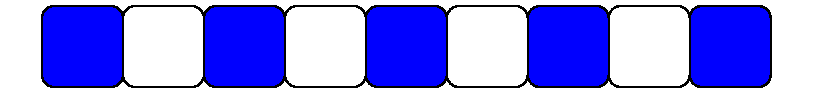
\includegraphics[scale=0.7]{figuras/loop_perfo.pdf}
    \fonte{}
    \addcontentsline{loge}{figure}{\protect\numberline{\thefigure}Modelo de execução do algoritmo de perforação de laço.}
\end{figure}

\subsection{Memoização}\label{subsec:memo}

A memoização é tradicionalmente uma técnica associada à programação dinâmica que utiliza uma \textit{cache} de resultados para acelerar a execução de determinadas computações. Seu princípio consiste em armazenar os resultados de chamadas já realizadas, indexados pelas entradas correspondentes. Assim, quando a função é invocada novamente com os mesmos parâmetros, o valor previamente calculado é retornado diretamente, evitando a repetição da computação~\cite{michie1968}.

A memoização aproximada, também chamada de memoização temporal, estende esse conceito ao considerar tempo de execução e localização como critérios adicionais. Sua ideia principal é explorar o fato de que chamadas consecutivas a uma mesma função tendem a produzir resultados similares~\cite{tziantzioulis2018}.

Na prática, as saídas são armazenadas em uma estrutura de dados e reutilizadas seletivamente em chamadas subsequentes. As estratégias de \textit{cache} podem variar, incluindo modelos globais, específicos por função ou mesmo dependentes de contexto. O reuso é normalmente controlado por um limiar de tolerância, que avalia a variação das saídas: se os resultados permanecerem estáveis dentro desse limite, a função é considerada estável e, portanto, pode ser memoizada~\cite{tziantzioulis2018}.

\subsection{Aproximação de ponto flutuante}\label{subsec:pontoFlut}

A representação de números reais por meio de números de ponto flutuante envolvem aproximação por padrão devido a impossibilidade de representar valores contínuos, se torna impossível representar um número infinito com um número finito de \textit{bits}~\cite{monniaux2008}. Por esse motivo aritmética com números de ponto flutuante usualmente introduzem erros de aproximação que variam conforme a ordem de execução dessas operações, resultando em um valor completamente diferente do esperado. Um exemplo disso pode ser obervado na \autoref{fig:floatPoint}.

\begin{figure}[htb]
    \caption{Erro introduzido na aritmética de ponto flutuante.}
    \label{fig:floatPoint}
    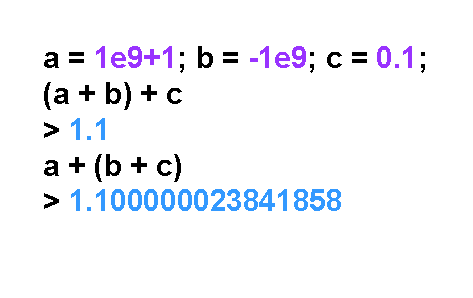
\includegraphics[scale=0.7]{figuras/fastmath.pdf}
    \fonte{}
    \addcontentsline{loge}{figure}{\protect\numberline{\thefigure}Erro introduzido na aritmética de ponto flutuante.}
\end{figure}

Para reduzir este tipo de problema, compiladores usualmente evitam aplicar certas otimizações que podem amplificar o erro nesse tipo de operação. Porém, alguns compiladores como é o caso do \texttt{Clang} e o \texttt{GCC}, suportam a opção \texttt{--fast-math} que passa a permitir a aplicação dessas otimizações em todo um módulo de compilação~\cite{gccffast, clangffast}. E de maneira similar o \texttt{MSVC} suporta o uso da diretiva de compilação \texttt{\#pragma float\_control} para definir regiões do código que permitem o uso dessas otimizações em certas regiões decódigo~\cite{msvcfast}.

\subsection{Descarte de tarefas}\label{subsec:descTar}

O descarte de tarefas é um conceito abrangente que engloba diferentes técnicas de aproximação, incluindo, em alguns casos, a própria perforação de laço. Sua ideia central baseia-se em computações que podem ser divididas em unidades menores, chamadas tarefas, das quais uma parte delas é descartada~\cite{mittal2016}.

As implementações dessa técnica costumam adotar uma taxa de descarte, que define a fração de tarefas a serem eliminadas durante a execução do programa. A \autoref{fig:perfoMod} também pode ser utilizada para ilustrar esse mecanismo: os blocos brancos representam tarefas descartadas, enquanto os blocos azuis indicam as tarefas efetivamente executadas.

\section{Computação paralela}\label{sec:compParalela}

A \gls{cp} é uma área da computação que busca explorar arquiteturas modernas, cada vez mais baseadas em processadores \textit{multicore}. Esse conceito pode ser melhor compreendido a partir da taxonomia de Flynn~\cite{flynn1972}, que classifica as arquiteturas de computadores de acordo com o fluxo de instruções e de dados:

\begin{itemize}
    \item \textbf{SISD (\textit{Single Instruction, Single Data stream}):} Instrução única que atua sobre uma única fonte de dados.
    \item \textbf{SIMD (\textit{Single Instruction, Multiple Data stream}):} Instrução única que é aplicada simultaneamente a múltiplos dados.
    \item \textbf{MISD (\textit{Multiple Instructions, Single Data stream}):} Múltiplas instruções atuando sobre uma mesma fonte de dados.
    \item \textbf{MIMD (\textit{Multiple Instructions, Multiple Data stream}):} Múltiplas instruções atuando em paralelo sobre múltiplas fontes de dados.
\end{itemize}

Dentro desse modelo, o paralelismo pode ser explorado de diferentes maneiras. No nível do processador, técnicas como \textit{pipeline}, predição de desvios (\textit{branch prediction}) e escalonamento dinâmico permitem dividir o código em pequenas unidades que podem ser executadas simultaneamente.

Algumas arquiteturas foram além e incorporaram extensões \gls{simd}, permitindo a utilização de processadores vetoriais capazes de realizar a mesma operação sobre múltiplos elementos de um vetor unidimensional em um único ciclo de instrução. Em cenários mais especializados, como nas \glspl{gpu}, esse modelo é expandido para múltiplas dimensões de dados, possibilitando que milhares de operações sejam executadas em paralelo e tornando-as altamente adequadas para cargas de trabalho massivamente paralelizáveis~\cite{hennessy2017}. Outro mecanismo fundamental é o uso de \textit{threads}, que representam abstrações de execução em nível de software, permitindo que diferentes unidades computacionais operem concorrentemente em múltiplos processadores. Cada \textit{thread} possui seu próprio contexto de execução, mas pode compartilhar recursos como memória e dispositivos de entrada/saída, viabilizando desde o paralelismo de tarefas independentes até a cooperação em algoritmos que exploram granularidades mais finas~\cite{tanenbaum2015,hennessy2017}.

É nesse contexto que surge o OpenMP, uma \gls{api} projetada para estender C, C++ e Fortran com suporte à paralelização de aplicações por meio de anotações de código. Essas anotações especificam o como aquela região de código deve ser executada. Seu modelo de programação permite explorar automaticamente diferentes formas de paralelismo, seja pelo \textit{offloading} para \glspl{gpu}, pelo uso de múltiplas \textit{threads}, ou ainda pela vetorização via \gls{simd}, aproveitando as unidades vetoriais das arquiteturas modernas~\cite{mattson2019}.

\begin{figure}[htb]
    \caption{Arquitetura do \texttt{OpenMP}.}
    \label{fig:ompArchitecture}
    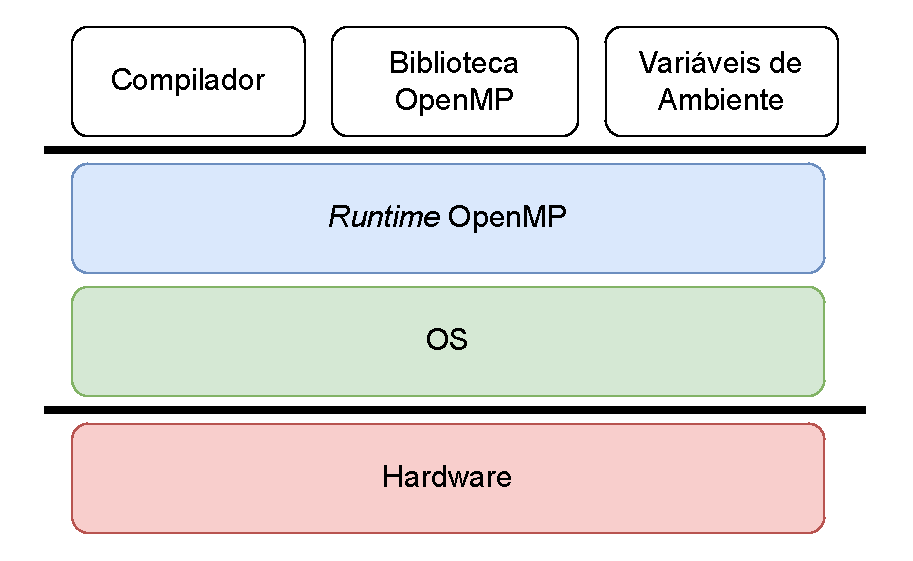
\includegraphics[scale=0.7]{figuras/omp_architecture.pdf}
    \fonte{}
    \addcontentsline{loge}{figure}{\protect\numberline{\thefigure}Arquitetura do \texttt{OpenMP}.}
\end{figure}

O OpenMP é estruturado em uma arquitetura em camadas, composta por anotações de código, suporte da \textit{runtime} e configurações do ambiente de execução, conforme ilustrado na FIGURA. Esse modelo permite ao programador controlar diversos aspectos da execução por meio de diretivas e chamadas à biblioteca, como a definição do número de \textit{threads} em uma região paralela e a escolha do comportamento do escalonador. Dessa forma, o OpenMP oferece um controle flexível sobre o paralelismo do programa.

A \autoref{code:produtoVet} apresenta a implementação sequencial de um produto escalar entre vetores. A paralelização utilizando a biblioteca \texttt{pthreads}, apresentada no \autoref{code:produtoThread}, exige a criação explícita de \textit{threads}, gerenciamento de regiões de memória e sincronização dos resultados parciais. Em contraste, o \autoref{code:produtoOmp} implementado com o OpenMP, evidencia a simplicidade proporcionada pelas diretivas: uma única anotação é suficiente para paralelizar o laço de cálculo, delegando à \textit{runtime} a criação e sincronização das \textit{threads}.

\begin{sourcecode}[htb]\caption{\label{code:produtoVet}Estrutura de um laço canônico}
    \begin{lstlisting}[frame=single, language=C++]
        for (int i = 0; i < N; i++) {
            result += a[i] * b[i];
        }
    \end{lstlisting}
    \fonte{}
\end{sourcecode}

\begin{sourcecode}[htb]\caption{\label{code:produtoThread}Estrutura de um laço canônico}
    \begin{lstlisting}[frame=single, language=C++]
        void *compute_partial_dot(void *arg) {
            ThreadArgs *args = (ThreadArgs *)arg;
            args->partial_sum = 0.0;
            
            for (int i = args->start; i < args->end; i++) {
                args->partial_sum = 0.0; += args->a[i] * args->b[i];
            }

            return NULL;
        }

    ...

    pthread_t threads[NUM_THREADS];
    ThreadArgs args[NUM_THREADS];
    result = 0.0;
    chunk_size = N / NUM_THREADS;

    for (int i = 0; i < NUM_THREADS; i++) {
        args[i].start = i * chunk_size;
        args[i].end = (i == NUM_THREADS - 1) ? N : (i + 1) * chunk_size;
        args[i].a = a;
        args[i].b = b;
        pthread_create(&threads[i], NULL, compute_partial_dot, &args[i]);
    }

    for (int i = 0; i < NUM_THREADS; i++) {
        pthread_join(threads[i], NULL);
        result += args[i].partial_sum;    
    }
    \end{lstlisting}
    \fonte{}
\end{sourcecode}

\begin{sourcecode}[htb]\caption{\label{code:produtoOmp}Estrutura de um laço canônico}
    \begin{lstlisting}[frame=single, language=C++]
        #pragma omp parallel for reduction(+ : result)
        for (int i = 0; i < N; i++) {
            result += a[i] * b[i];
        }
    \end{lstlisting}
    \fonte{}
\end{sourcecode}

Tipicamente, uma diretiva OpenMP é aplicada a um laço para indicar que ele pode ser executado em paralelo. Durante a compilação, esse bloco de código é isolado e transformado em tarefas, enquanto a \textit{runtime} prepara as estruturas necessárias para o modelo \textit{fork-join}. Por exemplo, a diretiva \texttt{\#pragma omp parallel} cria um time de \textit{threads}, cada uma executando uma cópia do código anotado. O compilador gerencia variáveis privadas, memória de pilha e pontos de sincronização automaticamente. Ao final, as \textit{threads} são reunificadas (\textit{joined}), e a execução retorna ao fluxo sequencial. Essa abordagem permite paralelizar regiões de código com esforço reduzido de gerenciamento, mantendo controle sobre sincronização e compartilhamento de dados~\cite{mattson2019}.

\begin{figure}[htb]
    \caption{Modelo \textit{fork-join} de execução do \texttt{OpenMP}.}
    \label{fig:ompExec}
    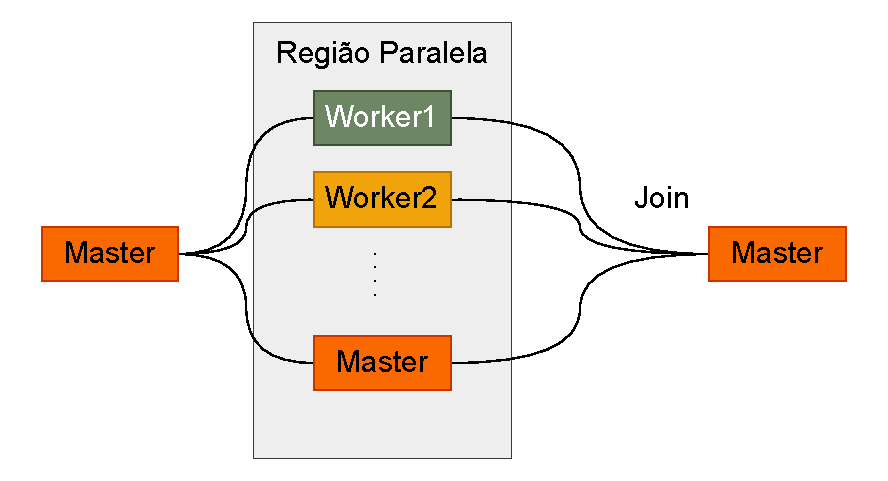
\includegraphics[scale=0.7]{figuras/omp_exec.pdf}
    \fonte{}
    \addcontentsline{loge}{figure}{\protect\numberline{\thefigure}Modelo \textit{fork-join} de execução do \texttt{OpenMP}.}
\end{figure}

O modelo \textit{fork-join} pode ser observado de forma esquemática na \autoref{fig:ompExec}. Nele, a \textit{runtime} cria múltiplas \textit{threads} para a execução paralela, que são sincronizadas ao final, restando apenas a \textit{thread} principal para continuar a execução sequencial. O OpenMP também suporta regiões paralelas aninhadas, possibilitando hierarquias de paralelismo.

\section{Trabalhos Relacionados}\label{sec:trabRelac}

Esta seção apresenta arcabouços baseados no paradigma de \gls{ca} que implementam suporte em nível de linguagem de programação, especialmente aqueles que utilizam anotações de código e mecanismos de execução em \textit{runtime}. Os arcabouços e aplicações selecionados buscam oferecer ao desenvolvedor maior controle sobre as técnicas utilizadas e sobre as regiões de código que podem ser aproximadas.

O ACCEPT~\cite{sampson2015} (Approximate C Compiler for Energy and Performance Trade-Off) é um arcabouço implementado sobre a infraestrutura do LLVM, que introduz a palavra-chave \texttt{ACCEPT} na sintaxe das linguagens C/C++. Essa palavra-chave permite diferenciar regiões de código aproximadas daquelas que devem ser executadas de forma precisa. O arcabouço também implementa etapas de análise para verificar a possibilidade de aproximação dessas regiões, avaliando não apenas a validade das transformações, mas também viabilizando a aplicação de diferentes técnicas de otimização aproximada, de maneira análoga ao funcionamento de um compilador paralelizador.

A infraestrutura do ACCEPT permite, por meio de anotações de código e análises estáticas e dinâmicas, identificar regiões de código potencialmente aproximáveis. Essas regiões podem ser exploradas para aplicar técnicas como perforação de laço, elisão de sincronização e até mesmo o uso de redes neurais em \textit{hardware} para estimar saídas. Além disso, o arcabouço incorpora um \textit{autotuner} que utiliza métricas fornecidas pelo usuário para avaliar se as aproximações aplicadas mantêm a qualidade de saída dentro dos limites esperados, garantindo que o programa não apresente falhas durante a execução.

Vassiliadis et al.~\cite{vassiliadis2015} propõem uma extensão ao OpenMP que incorpora suporte à \gls{ca} no modelo de programação baseado em tarefas. Em sua proposta, o programador pode especificar funções aproximadas alternativas que podem ser escolhidas em tempo de execução para substituir versões precisas de determinadas tarefas. Assim, parte das tarefas é executada de forma exata, enquanto outras utilizam versões aproximadas, reduzindo o consumo energético e mantendo a qualidade de acordo com limites definidos pelo usuário.

O arcabouço também introduz um mecanismo de barreira para garantir que uma fração mínima das execuções alcance o grau de acurácia desejado. Para gerenciar essa execução, são propostas duas políticas no runtime: \textit{Global Task Buffering} (GTB), que toma decisões informadas a partir da análise conjunta de todas tarefas pendentes, e a \textit{Local Queue History} (LQH), baseada no histórico local de filas, em que cada \textit{worker} decide de maneira autônoma o nível de aproximação com base nas execuções anteriores.

Lashgar et al.~\cite{lashgar2018} propõem a integração da técnica de perforação de laço ao \texttt{OpenACC} com o objetivo de melhorar o desempenho, executando apenas um subconjunto das iterações do laço. Dessa forma, parte das saídas é calculada de maneira exata, enquanto o restante é aproximado. Para mitigar os impactos dessa abordagem na precisão e no tempo de execução dentro do \texttt{OpenACC}, os autores introduzem um mecanismo de correção implementado diretamente no kernel. Esse mecanismo identifica as saídas ausentes e aplica estratégias como a cópia ou a média dos valores vizinhos já computados, a fim de estimar as entradas faltantes.

O HPAC~\cite{parasyris2021} é um arcabouço de técnicas de computação aproximada voltadas para aplicações HPC, implementado sobre a infraestrutura do LLVM. Ele utiliza anotações de código \texttt{pragma} para C/C++, permitindo a definição de regiões de código aproximadas, e se destaca por sua interoperabilidade com o OpenMP. As técnicas principais incluem perforação de laço e memoização aproximada, e o arcabouço fornece ainda uma ferramenta de análise que permite ao usuário anotar múltiplas regiões de código e avaliar a qualidade dos resultados obtidos para cada configuração.

O HPAC-Offload~\cite{fink2023} é uma extensão do HPAC~\cite{parasyris2021} voltada para aplicações em GPU, que adapta sua arquitetura para lidar com as limitações do modelo de memória e paralelismo dessas plataformas. Assim como no HPAC, as técnicas implementadas incluem perforação de laço e memoização aproximada, mas com um gerenciamento de memória consciente da GPU: os dados internos de AC são armazenados na memória compartilhada do bloco, permitindo reutilização entre threads ativas sem sobrecarregar a memória global. O arcabouço também define níveis hierárquicos de aproximação (\textit{thread}, \textit{warp} e bloco) para evitar divergência e deadlocks.

Em contraste com outros trabalhos, nossa abordagem baseia-se na extensão do próprio framework \texttt{OpenMP}, modificando sua \textit{runtime} e alterando suas diretivas de compilação para oferecer suporte nativo a técnicas de \gls{ca}. Ao incorporar o controle de aproximação diretamente no \texttt{OpenMP}, habilitamos o escalonamento e a execução de tarefas sem comprometer sua API. Essa integração não apenas simplifica a adoção de \gls{ca} em computação paralela, como também abre caminho para uma exploração mais ampla e eficaz da aproximação em aplicações que já utilizam o OpenMP. A Tabela~\ref{tab:trabComp}, apresenta um breve resumo e comparação entre todos os trabalhos citados.

\begin{table}[htb]
    \centering
    \caption{Resumo e comparação entre os trabalhos citados}
    \begin{tabular}{|p{2.3cm}|p{3cm}|p{2cm}|p{3cm}|p{4cm}|}
        \hline
        \textbf{Trabalho}                         & \textbf{Linguagem / Infraestrutura} & \textbf{Suporte a Paralelismo} & \textbf{Técnicas de Aproximação}                                                                        & \textbf{Diferenciais}                                                                                                                                                      \\
        \hline
        ACCEPT~\cite{sampson2015}                 & C/C++, LLVM                         & Sequencial e paralelo          & Perforação de laço, elisão de sincronização e redes neurais em \textit{hardware}                        & Validação de aproximações em tempo de execução; Aplicação de múltiplas técnicas de otimização                                                                              \\
        \hline
        Vassiliadis et al.~\cite{vassiliadis2015} & C/C++, OpenMP                       & Paralelismo baseado em tarefas & Funções aproximadas                                                                                     & Controle de acurácia; Decisões globais e locais para aproximação                                                                                                           \\
        \hline
        Lashgar et al.~\cite{lashgar2018}         & C/C++, OpenACC                      & Paralelismo em laço            & Perforação de laço                                                                                      & Estima valores ausentes para manter precisão em laços aproximados                                                                                                          \\
        \hline
        HPAC~\cite{parasyris2021}                 & C/C++, LLVM, OpenMP                 & Regiões paralelas              & Perforação de laço, memoização aproximada                                                               & Interoperabilidade com OpenMP; Análise de múltiplas regiões de código                                                                                                      \\
        \hline
        HPAC-Offload~\cite{fink2023}              & C/C++, LLVM, OpenMP                 & Paralelismo via GPU            & Perforação de laço, memoização aproximada                                                               & Interoperabilidade com OpenMP; Hierarquia de aproximação em GPU                                                                                                            \\
        \hline
        \textbf{Este Trabalho}                    & \textbf{C/C++, LLVM, OpenMP}        & \textbf{Regiões paralelas}     & \textbf{Perforação de laço, memoização aproximada, aproximação em ponto flutuante, descarte de tarefas} & \textbf{Integração direta com OpenMP; Combina análise em tempo de compilação e decisões em tempo de execução; Aplica múltiplas técnicas de aproximação visando desempenho} \\
        \hline
    \end{tabular}
    \fonte{}
    \label{tab:trabComp}
\end{table}


\section{Trabalhos relacionados}\label{sec:trabRelac}

Ao longo dos anos uma grande variedade de \textit{frameworks} e metodologias vem sendo prosposta para suportar \gls{ca} em diferentes níveis de abstração. Os trabalhos apresentados nessa seção buscam prover técnicas em nível de \textit{runtime} e também buscam prover um equilibrío entre ganhos eficiência e qualidade de saída, usualmente utilizando estratégias de estatistíca, adaptação em tempo \textit{runtime} ou anotações em nível de linguagem de programação.

\texttt{ApproxHadoop}~\cite{goiri2015} é uma extensãoa ao \texttt{Hadoop} para suportar o descarte de seletivo tarefas (\textit{task dropping}) no \texttt{MapReduce}. Por meio de um mecanismo de amostragem dos dados de entrada, a extensão visa reduzir o tempo de execução e o consumo de recursos ao evitar o processamento completo dos dados, sem perder de vista a utilidade prática dos resultados. Além disso, o sistema integra métodos estatísticos que calculam limites de erro, fornecendo garantias quantitativas sobre a precisão das respostas aproximadas.

Rinard~\cite{rinard2006} propôs uma metodologia de particionamento da computação em tarefas que podem ser descartadas, seja em resposta a falhas ou de forma deliberada para melhorar o desempenho. Em sua abordagem a aplicação é decomposta em tarefas, que são analisdas para distinguir as essenciais daquelas que podem ser descartas, isso é feito por meio de um teste onde o programa é executado e a \textit{runtime} insere falhas de maneira proposital para verificar se o programa suporta aquela falha ou não, e também é usado um modelo de regrassão obtido por amostragem repetida para prever os efeitos dessas omissões.

Lashgar et al.~\cite{lashgar2018} propõem a integração da técnica de perforação de laço ao \texttt{OpenACC} com o objetivo de melhorar o desempenho, executando apenas um subconjunto das iterações do laço. Dessa forma, parte das saídas é calculada de maneira exata, enquanto o restante é aproximado. Para mitigar os impactos dessa abordagem na precisão e no tempo de execução dentro do \texttt{OpenACC}, os autores introduzem um mecanismo de correção implementado diretamente no kernel. Esse mecanismo identifica as saídas ausentes e aplica estratégias como a cópia ou a média dos valores vizinhos já computados, a fim de estimar as entradas faltantes.

O \texttt{Sculptor}~\cite{li2018} é um \textit{framework} geral para perforação de laço dinâmica e seletiva, que avança em relação às técnicas tradicionais ao permitir aproximações em nível fino, tanto no nível de instruções individuais quanto no nível das iterações. Diferentemente das abordagens clássicas, que pulam um subconjunto fixo de iterações de forma uniforme, o \texttt{Sculptor} seleciona dinamicamente quais instruções devem ser ignoradas dentro dos laços e ajusta, em tempo de execução, as taxas de perfuração e os pontos de início de acordo com o comportamento do programa. Ele emprega uma \textit{pipeline} de otimizações do compilador em múltiplas etapas, capaz de identificar instruções com baixo impacto na precisão, mas alto potencial de ganho de desempenho, transformando os laços de forma adequada. Além disso, o \textit{framework} inclui escalonadores dinâmicos que adaptam o grau de agressividade da perfuração entre diferentes contextos de chamada e fases do laço.

O \texttt{SampleMine}~\cite{jiang2022} é um \textit{framework} que acelera a mineração de padrões em subgrafos aplicando perforação de laço nos laços aninhados usados na exploração dos subgrafos. Ele introduz uma técnica de expansão baseada em dois vértices, na qual cada passo adiciona dois vértices ao subgrafo, reduzindo a complexidade computacional em comparação com os métodos tradicionais, que acrescentam apenas um vértice por iteração.

Vassiliadis et al.~\cite{vassiliadis2015} propõem um \textit{framework} que introduz um modelo de programação baseado em tarefas, no qual os desenvolvedores podem anotar cada tarefa com um nível de significância e, opcionalmente, fornecer versões aproximadas. A \textit{runtime} decide dinamicamente quais tarefas devem ser executadas de forma precisa ou aproximada, de acordo com as restrições de qualidade definidas pelo usuário. Duas políticas de execução são implementadas: \textit{Global Task Buffering (GTB)}, que armazena tarefas para permitir decisões globalmente informadas, e \textit{Local Queue History (LQH)}, que se baseia no histórico local das tarefas para decisões descentralizadas e mais rápidas.

\texttt{HPAC}~\cite{parasyris2021} é um \textit{framework} que integra suporte de compilador e de tempo de execução para habilitar computação aproximada em aplicações de \gls{hpc} utilizando OpenMP. Ele permite que os desenvolvedores anotem regiões de código com diretivas de aproximação e avaliem o equilibrío entre precisão e desempenho. O \texttt{HPAC} oferece suporte a técnicas como perforação de laço, memoização de entrada e saída, além de fornecer ferramentas para avaliar o impacto dessas técnicas na execução paralela.

%% Formatação de páginas de elementos pós-textuais
\postextual%% Não comente esta linha

%% Arquivos de referências
\arquivosdereferencias{%% Arquivos bibtex sem a extensão .bib e separados por vírgula - Não comente esta linha
  %./PosTexto/exemplos-referencias,%% Arquivo de referências - Comente para remover este item
  main%% Arquivo de referências - Comente para remover este item
}%% Não comente esta linha

%% Glossário
%\incluirglossario %% Comente para remover este item

%% Arquivos de apêndices
\begin{arquivosdeapendices}%% Os arquivos de apêndices devem se incluídos neste ambiente - Não comente esta linha
  %   %\partapendices%% Página de início dos apêndices - adiciona uma página com o título Apêndices
  %   %% Capítulo de exemplo
  %%%% APÊNDICE A
%%
%% Texto ou documento elaborado pelo autor, a fim de complementar sua argumentação, sem prejuízo da unidade nuclear do trabalho.

%% Título e rótulo de apêndice (rótulos não devem conter caracteres especiais, acentuados ou cedilha)
\chapter{Questionário de pesquisa}\label{cap:apendicea}

Quando houver necessidade pode-se apresentar como apêndice documento(s) auxiliar(es) e/ou complementar(es) como: legislação, estatutos, gráficos, tabelas, etc. Os apêndices são enumerados com letras maiúsculas: \autoref{cap:apendicea}, \autoref{cap:apendiceb}, etc.

No \latex\ apêndices são editados como capítulos. O comando \verb|\appendix| faz com que todos os capítulos seguintes sejam considerados apêndices.

Apêndices complementam o texto principal da tese com informações para leitores com especial interesse no tema, devendo ser considerados leitura opcional, ou seja, o entendimento do texto principal da tese não deve exigir a leitura atenta dos apêndices.

Apêndices usualmente contemplam provas de teoremas, deduções de fórmulas matemáticas, diagramas esquemáticos, gráficos e trechos de código. Quanto a este último, código extenso não deve fazer parte da tese, mesmo como apêndice. O ideal é disponibilizar o código na Internet para os interessados em examiná-lo ou utilizá-lo.

%% Título e rótulo de seção (rótulos não devem conter caracteres especiais, acentuados ou cedilha)
%\section{Título da Seção Secundária do Apêndice B}\label{sec:secaoapendicea}

%Exemplo de seção secundária em apêndice (\autoref{sec:secaoapendicea} do \autoref{cap:apendicea}).

%% Título e rótulo de seção (rótulos não devem conter caracteres especiais, acentuados ou cedilha)
%\subsection{Título da Seção Terciária do Apêndice B}\label{subsec:subsecaoapendicea}

%Exemplo de seção terciária em apêndice (\autoref{subsec:subsecaoapendicea} do \autoref{cap:apendicea}).

%% Título e rótulo de seção (rótulos não devem conter caracteres especiais, acentuados ou cedilha)
%\subsubsection{Título da seção quaternária do Apêndice B}\label{subsubsec:subsubsecaoapendicea}

%Exemplo de seção quaternária em apêndice (\autoref{subsubsec:subsubsecaoapendicea} do \autoref{cap:apendicea}).

%% Título e rótulo de seção (rótulos não devem conter caracteres especiais, acentuados ou cedilha)
%\paragraph{Título da seção quinária do Apêndice B}\label{para:paragraphapendicea}

%Exemplo de seção quinária em apêndice (\autoref{para:paragraphapendicea} do \autoref{cap:apendicea}).
%% Apêndice - Comente para remover este item
  %%%% APÊNDICE B
%%
%% Texto ou documento elaborado pelo autor, a fim de complementar sua argumentação, sem prejuízo da unidade nuclear do trabalho.

%% Título e rótulo de apêndice (rótulos não devem conter caracteres especiais, acentuados ou cedilha)
\chapter{Roteiro da entrevista}\label{cap:apendiceb}

\begin{table}[htb]%% Ambiente table
\caption{Orçamento dos materiais n.\textsuperscript{o} 1.}%% Legenda
\label{tab:tab3}%% Rótulo
\begin{tabularx}{\textwidth}{@{\extracolsep{\fill}}lrrr}%% Ambiente tabularx
\toprule
Material              & \multicolumn{1}{c}{Valor (R\$)} & \multicolumn{1}{c}{Quantidade}  & \multicolumn{1}{c}{Total (R\$)} \\ \midrule
Bomba centrífuga      & 2500,00                         & 01                              & 2500,00                         \\
Compressor rotativo   & 3000,00                         & 01                              & 3000,00                         \\
Manômetro diferencial & 450,00                          & 02                              & 900,00                          \\
Termopar              & 370,00                          & 02                              & 740,00                          \\
Válvula de esfera     & 43,00                           & 02                              & 86,00                           \\
Tubulação de PVC      & 10,00                           & 05                              & 50,00                           \\
Conexão de PVC        & 5,00                            & 10                              & 50,00                           \\ \midrule
                      &                                 & \multicolumn{1}{r}{Total (R\$)} & 7326,00                         \\ \bottomrule
\end{tabularx}
\fonte{}%% Fonte
\end{table}

\begin{table}[htb]%% Ambiente table
\caption{Orçamento dos materiais n.\textsuperscript{o} 2.}%% Legenda
\label{tab:tab4}%% Rótulo
\begin{tabularx}{\textwidth}{@{\extracolsep{\fill}}lrrr}%% Ambiente tabularx
\toprule
Material              & \multicolumn{1}{c}{Valor (R\$)} & \multicolumn{1}{c}{Quantidade}  & \multicolumn{1}{c}{Total (R\$)} \\ \midrule
Bomba centrífuga      & 2700,00                         & 01                              & 2700,00                         \\
Compressor rotativo   & 2950,00                         & 01                              & 2950,00                         \\
Manômetro diferencial & 515,00                          & 02                              & 1030,00                         \\
Termopar              & 350,00                          & 02                              & 700,00                          \\
Válvula de esfera     & 40,00                           & 02                              & 80,00                           \\
Tubulação de PVC      & 8,00                            & 05                              & 40,00                           \\
Conexão de PVC        & 6,00                            & 10                              & 60,00                           \\ \midrule
                      &                                 & \multicolumn{1}{r}{Total (R\$)} & 7560,00                         \\ \bottomrule
\end{tabularx}
\fonte{}%% Fonte
\end{table}

\begin{table}[htb]%% Ambiente table
\caption{Orçamento dos materiais n.\textsuperscript{o} 3.}%% Legenda
\label{tab:tab5}%% Rótulo
\begin{tabularx}{\textwidth}{@{\extracolsep{\fill}}lrrr}%% Ambiente tabularx
\toprule
Material              & \multicolumn{1}{c}{Valor (R\$)} & \multicolumn{1}{c}{Quantidade}  & \multicolumn{1}{c}{Total (R\$)} \\ \midrule
Bomba centrífuga      & 2600,00                         & 01                              & 2600,00                         \\
Compressor rotativo   & 3100,00                         & 01                              & 3100,00                         \\
Manômetro diferencial & 500,00                          & 02                              & 1000,00                         \\
Termopar              & 400,00                          & 02                              & 800,00                          \\
Válvula de esfera     & 45,00                           & 02                              & 90,00                           \\
Tubulação de PVC      & 12,00                           & 05                              & 60,00                           \\
Conexão de PVC        & 5,00                            & 10                              & 50,00                           \\ \midrule
                      &                                 & \multicolumn{1}{r}{Total (R\$)} & 7700,00                         \\ \bottomrule
\end{tabularx}
\fonte{}%% Fonte
\end{table}
%% Apêndice - Comente para remover este item
\end{arquivosdeapendices}%% Não comente esta linha


% \begin{apendicesenv}%% Ambiente apendicesenv

% \partapendices
% \chapter{Ola}

% \lipsum[55-56]

% \end{apendicesenv}

%% Arquivos de anexos
\begin{arquivosdeanexos}%% Os arquivos de anexos devem se incluídos neste ambiente - Não comente esta linha
  %\partanexos%% Página de início dos anexos - adiciona uma página com o título Anexos

  %%%% ANEXO A
%%
%% Texto ou documento não elaborado pelo autor, que serve de fundamentação, comprovação e ilustração.

%% Título e rótulo de anexo (rótulos não devem conter caracteres especiais, acentuados ou cedilha)
\anexos
\chapter{Lei N\texorpdfstring{.\textsuperscript{o}}{o.} 9.610, de 19 de Fevereiro de 1998}\label{cap:anexoa}

\centerline{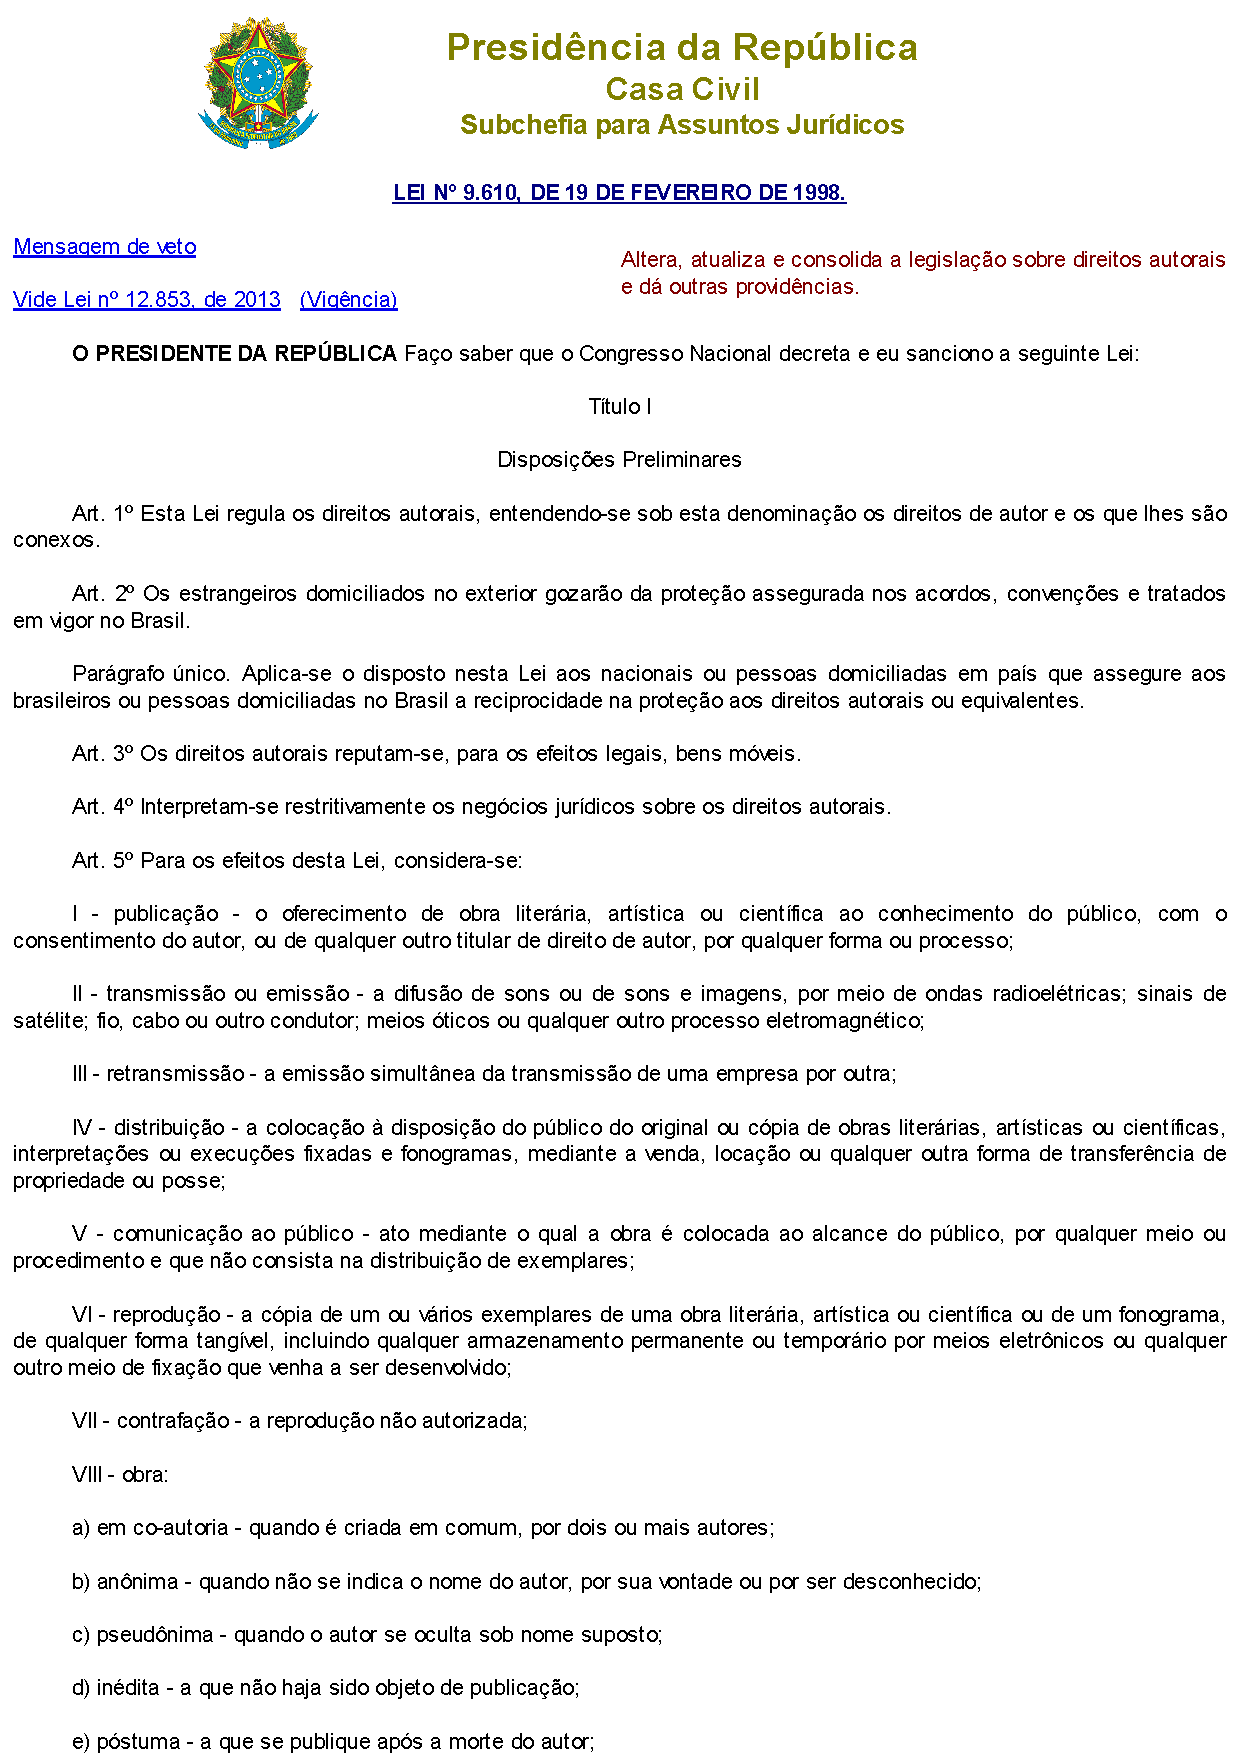
\includegraphics[width=\textwidth]{./PosTexto/Ilustracoes/lei-n9610-p1}}%% Imagem (Dimensões e localização)

\centerline{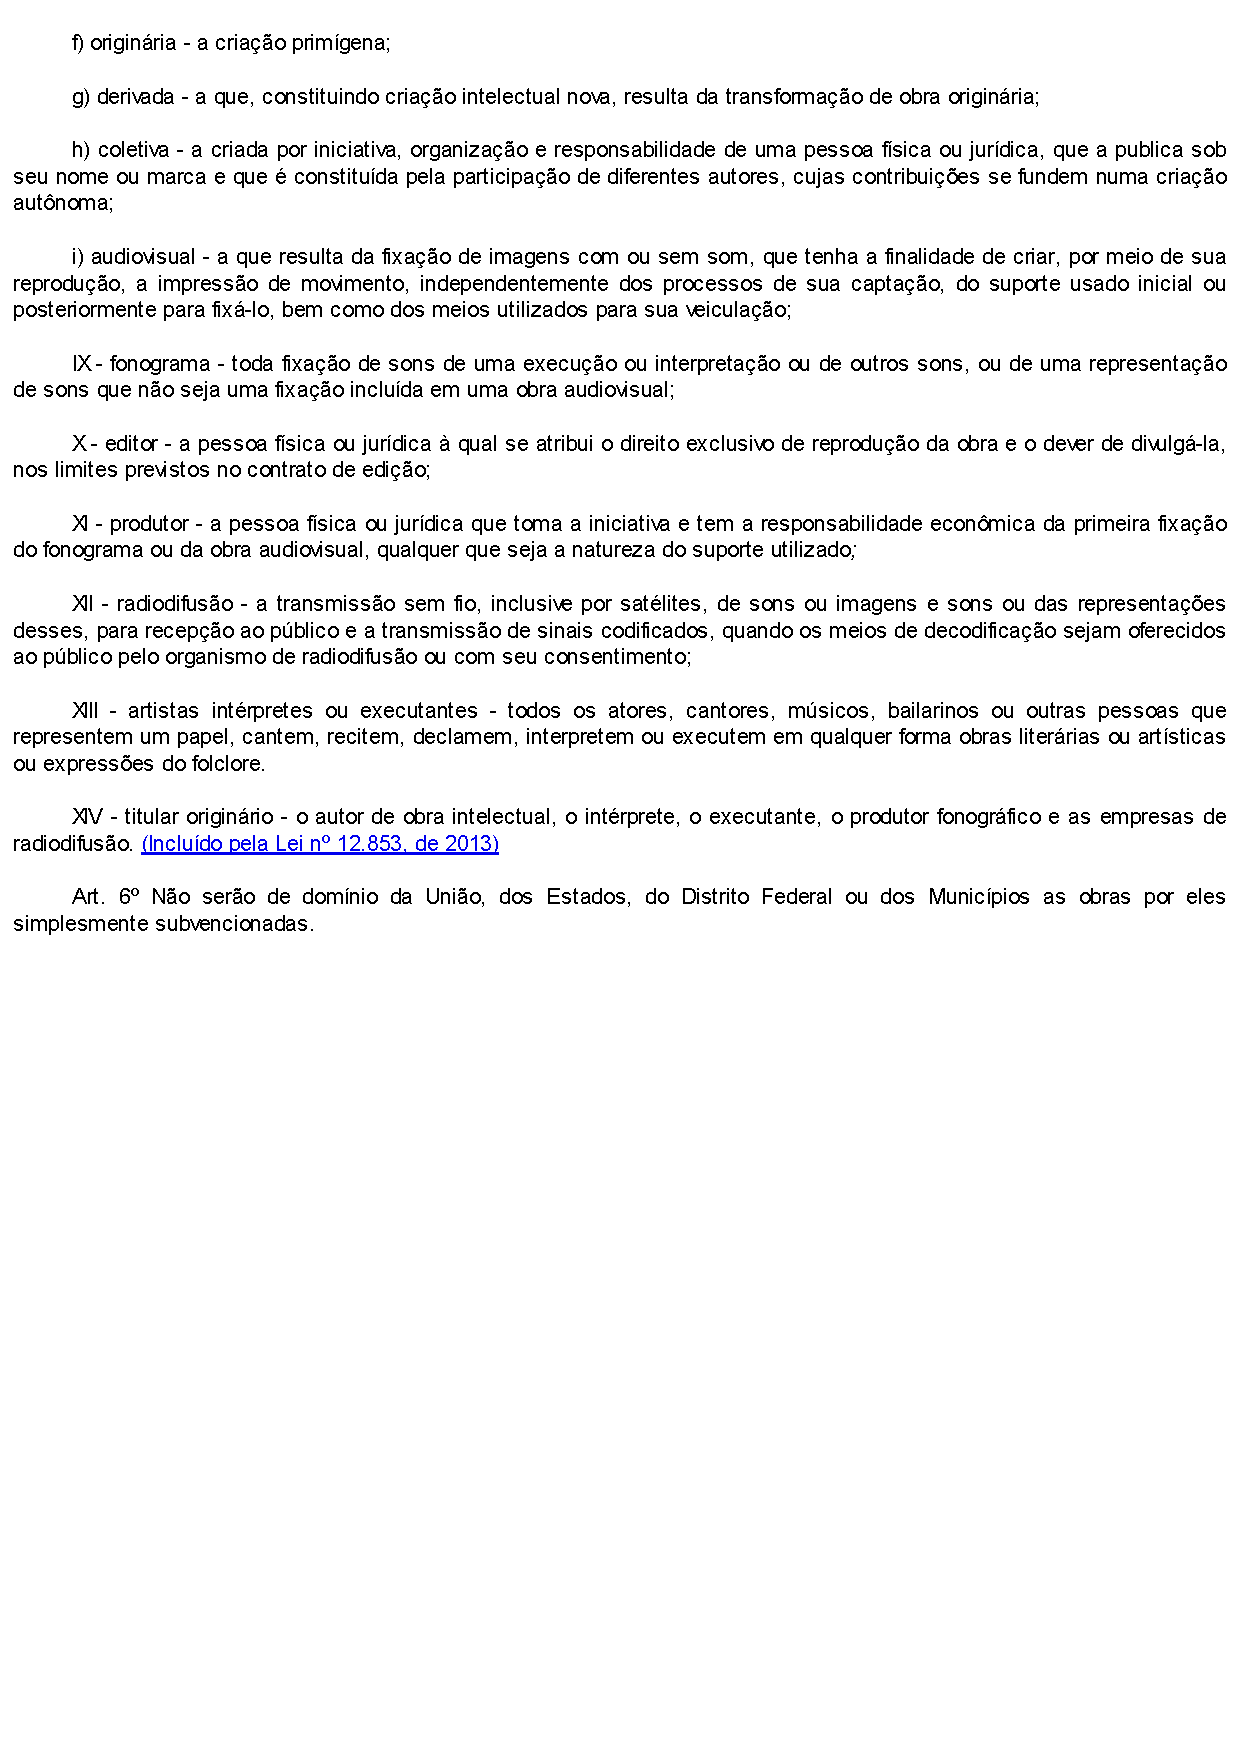
\includegraphics[width=\textwidth]{./PosTexto/Ilustracoes/lei-n9610-p2}}%% Imagem (Dimensões e localização)
%% Anexo - Comente para remover este item
  %%%% ANEXO B
%%
%% Texto ou documento não elaborado pelo autor, que serve de fundamentação, comprovação e ilustração.

%% Título e rótulo de anexo (rótulos não devem conter caracteres especiais, acentuados ou cedilha)
% \chapter{Normas para elaboração de trabalhos acadêmicos}\label{cap:anexob}%% Anexo - Comente para remover este item
\end{arquivosdeanexos}%% Não comente esta linha

%% Índice - Adiciona um índice remissivo.
%\incluirindice%% Comente para remover este item

%% Fim do documento
\end{document}%% Não comente esta linha
